\documentclass{article}
\usepackage{graphicx} 
\usepackage{wrapfig}
\usepackage{filecontents}
\usepackage{siunitx}
\usepackage[table]{xcolor}
\usepackage{float}
\usepackage{hyperref}

\usepackage{color} % balíček pro obarvování textů
\usepackage{xcolor}  % zapne možnost používání barev, mj. pro \definecolor
\usepackage{pgfplots} % http://www.chiark.greenend.org.uk/doc/texlive-doc/latex/pgfplots/pgfplots.pdf

\usepackage{multirow}
\usepackage{caption}

\captionsetup[figure]{name=obr}


\ifnum 0\ifxetex 1\fi\ifluatex 1\fi=0 % if pdftex
  \usepackage[T1]{fontenc}
  \usepackage[utf8]{inputenc}
\else % if luatex or xelatex
  \ifxetex
    \usepackage{mathspec}
  \else
    \usepackage{fontspec}
  \fi
  \defaultfontfeatures{Ligatures=TeX,Scale=MatchLowercase}
\fi
\usepackage[total={175mm,230mm}, top=23mm, left=20mm, includefoot]{geometry}
\hypersetup{
    colorlinks,
    linkcolor={blue!50!black},
    citecolor={green!50!black},
    urlcolor={blue!80!black}
}
% \definecolor{fialova}{RGB}{ 255, 000, 255}
\definecolor{color-si1}{RGB}{ 255, 000, 000}
\definecolor{color-si2}{RGB}{ 251, 130, 032}

\definecolor{color-ge1}{RGB}{ 000, 255, 000}
\definecolor{color-ge2}{RGB}{ 032, 251, 160}

\definecolor{color-inp1}{RGB}{ 000, 000, 255}
\definecolor{color-inp2}{RGB}{ 160, 032, 251}

\definecolor{color-geas1}{RGB}{ 225, 225, 000}
\definecolor{color-geas2}{RGB}{ 225, 225, 100}

\definecolor{sedak}{RGB}{ 100, 100, 100}


\newcommand \obr[1]
{ obr.~\ref{#1}}

\newcommand \tab[1]
{ tab.~ß\ref{#1}}


\begin{document}

% 
\pagestyle{empty}

\definecolor{color_29791}{rgb}{0,0,0}
\begin{figure}[H]
    \hspace{-13mm}
    \begin{minipage}[t]{\textwidth}
        \vspace{-20mm}
        \begin{tikzpicture}[overlay]
            \path(0pt,0pt);
        \end{tikzpicture}
        \begin{picture}(-5,0)(2.5,0)
            \put(123.656,-82.75397){\fontsize{18}{1}\usefont{T1}{ptm}{m}{n}\selectfont\color{color_29791}VYSOKÉ UČENÍ TECHNICKÉ V BRNĚ}
            \put(76.296,-104.785){\fontsize{13}{1}\usefont{T1}{ptm}{m}{n}\selectfont\color{color_29791}FAKULTA  ELEKTROTECHNIKY A KOMUNIKAČNÍCH TECHNOLOGIÍ}
            \put(198.447,-128.5339){\fontsize{16}{1}\usefont{T1}{cmr}{b}{n}\selectfont\color{color_29791}Ústav elektrotechnologie}
            \put(156.848,-278.1589){\fontsize{14}{1}\usefont{T1}{ptm}{m}{n}\selectfont\color{color_29791}LABORATORNÍ CVIČENÍ Z PŘEDMĚTU}
            \put(108.123,-300.2579){\fontsize{14}{1}\usefont{T1}{cmr}{b}{n}\selectfont\color{color_29791}VYBRANÉ PARTIE Z OBNOVITELNÝCH ZDROJŮ A}
            \put(173.123,-320.2579){\fontsize{14}{1}\usefont{T1}{cmr}{b}{n}\selectfont\color{color_29791}UKLÁDÁNÍ ENERGIE (BPC-OZU)}
            \put(55.85,-421.25){\fontsize{14}{1}\usefont{T1}{cmr}{b}{n}\selectfont\color{color_29791}Číslo úlohy: 7}
            \put(55.85,-469.547){\fontsize{14}{1}\usefont{T1}{cmr}{b}{n}\selectfont\color{color_29791}Název úlohy: Využití termoelektrického jevu pro získávání energie}
            \put(23.9,-620.32){\fontsize{12}{1}\usefont{T1}{cmr}{b}{n}\selectfont\color{color_29791}Jméno a příjmení, ID:}
            \put(23.9,-637.119){\fontsize{12}{1}\usefont{T1}{cmr}{b}{n}\selectfont\color{color_29791}Tomáš Vavrinec, 240893}
            \put(186.95,-620.32){\fontsize{12}{1}\usefont{T1}{cmr}{b}{n}\selectfont\color{color_29791}Atmosférický tlak:}
            \put(186.95,-637.119){\fontsize{12}{1}\usefont{T1}{cmr}{b}{n}\selectfont\color{color_29791}1018 hPa}
            \put(293.25,-620.32){\fontsize{12}{1}\usefont{T1}{cmr}{b}{n}\selectfont\color{color_29791}Teplota okolí: }
            \put(293.25,-637.119){\fontsize{12}{1}\usefont{T1}{cmr}{b}{n}\selectfont\color{color_29791}21.7°C}
            \put(417.25,-620.32){\fontsize{12}{1}\usefont{T1}{cmr}{b}{n}\selectfont\color{color_29791}Relativní vlhkost:}
            \put(417.25,-637.119){\fontsize{12}{1}\usefont{T1}{cmr}{b}{n}\selectfont\color{color_29791}24.6\%}
            \put(23.9,-665.77){\fontsize{12}{1}\usefont{T1}{cmr}{b}{n}\selectfont\color{color_29791}Měřeno dne:}
            \put(23.9,-682.569){\fontsize{12}{1}\usefont{T1}{cmr}{b}{n}\selectfont\color{color_29791}25.2.2023}
            \put(186.95,-665.77){\fontsize{12}{1}\usefont{T1}{cmr}{b}{n}\selectfont\color{color_29791}Odevzdáno dne:}
            \put(293.25,-665.77){\fontsize{12}{1}\usefont{T1}{cmr}{b}{n}\selectfont\color{color_29791}Ročník, stud. skupina:}
            \put(293.25,-682.569){\fontsize{12}{1}\usefont{T1}{cmr}{b}{n}\selectfont\color{color_29791}2}
            \put(417.25,-665.77){\fontsize{12}{1}\usefont{T1}{cmr}{b}{n}\selectfont\color{color_29791}Kontrola:}
            \put(23.9,-703.42){\fontsize{12}{1}\usefont{T1}{cmr}{b}{n}\selectfont\color{color_29791}Spolupracovali:}
            \put(23.9,-720.219){\fontsize{12}{1}\usefont{T1}{cmr}{b}{n}\selectfont\color{color_29791}Kateřina Koudelková}
        \end{picture}
        \begin{tikzpicture}[overlay]
            \path(0pt,0pt);
            \draw[color_29791,line width=0.5pt]
            (20.4pt, -606.117pt) -- (20.4pt, -722.815pt)
            ;
            \draw[color_29791,line width=0.5pt]
            (183.45pt, -606.117pt) -- (183.45pt, -651.067pt)
            ;
            \draw[color_29791,line width=0.5pt]
            (183.45pt, -651.567pt) -- (183.45pt, -688.717pt)
            ;
            \draw[color_29791,line width=0.5pt]
            (289.75pt, -606.117pt) -- (289.75pt, -651.067pt)
            ;
            \draw[color_29791,line width=0.5pt]
            (289.75pt, -651.567pt) -- (289.75pt, -688.717pt)
            ;
            \draw[color_29791,line width=0.5pt]
            (413.75pt, -606.117pt) -- (413.75pt, -651.067pt)
            ;
            \draw[color_29791,line width=0.5pt]
            (413.75pt, -651.567pt) -- (413.75pt, -688.717pt)
            ;
            \draw[color_29791,line width=0.5pt]
            (544.9pt, -606.117pt) -- (544.9pt, -722.815pt)
            ;
            \draw[color_29791,line width=0.5pt]
            (20.15pt, -605.867pt) -- (545.15pt, -605.867pt)
            ;
            \draw[color_29791,line width=0.5pt]
            (20.65pt, -651.317pt) -- (544.65pt, -651.317pt)
            ;
            \draw[color_29791,line width=0.5pt]
            (20.65pt, -688.967pt) -- (544.65pt, -688.967pt)
            ;
            \draw[color_29791,line width=0.5pt]
            (20.15pt, -723.065pt) -- (545.15pt, -723.065pt)
            ;
            \draw[color_29791,line width=1.5pt]
            (15.75pt, -15.59998pt) -- (15.75pt, -729pt)
            ;
            \draw[color_29791,line width=1.5pt]
            (549.55pt, -15.59998pt) -- (549.55pt, -729pt)
            ;
            \draw[color_29791,line width=1.5pt]
            (15.75pt, -729pt) -- (549.55pt, -729pt)
            ;
            \draw[color_29791,line width=1.5pt]
            (15pt, -14.84998pt) -- (550.3pt, -14.84998pt)
            ;
        \end{tikzpicture}
    \end{minipage}
\end{figure}

\newpage
\pagestyle{plain}

\section*{Operační zesilovač}

\begin{figure}[H]
  \begin{minipage}[t]{1.1\textwidth}
    \vspace{10mm}
    \hspace{-0.05\textwidth}
    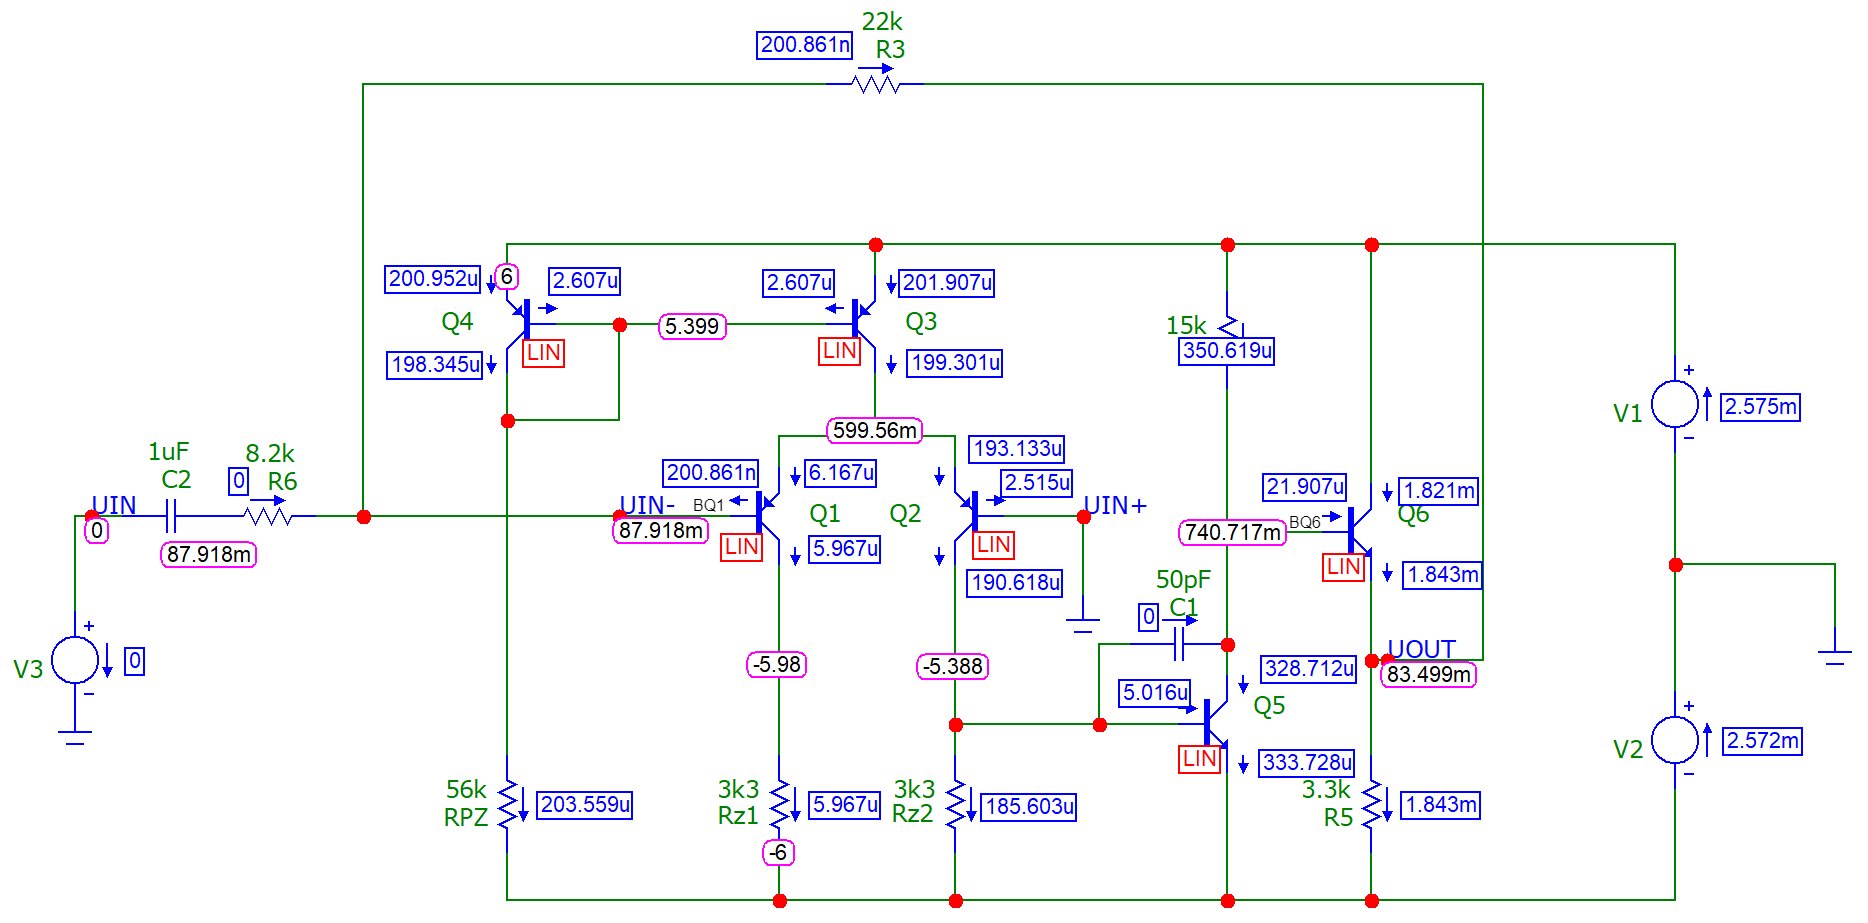
\includegraphics[width=\textwidth]{sim/bezporuch/sch.png}
    \caption[obr]{Schema zapojení bez poruchy s vyznačenými proudy a napětími}
    \label{sch-bezPoruch}
  \end{minipage}
\end{figure}

\begin{figure}[H]
  \begin{minipage}[t]{\textwidth}
    \begin{table}[H]
      \centering
      \vspace{-10mm}
      \begin{tabular}{|c|c|c|c|c|c|c|}
      \hline
      porucha	& \(U_{CQ3}\-[V]\)	& \(U_{BQ6}\-[V]\)	& \(U_{out}\-[V]\)	& \(U_{BQ1}\-[V]\)	& \(U_{RZ1}\-[V]\)	& \(U_{RZ2}\-[V]\) \\ \hline
      0	      & 0.58	            & 0.81	            & 0.172	            & 0.049	            & -5.32	            & -4.78            \\ \hline
      1	      & 0.58	            & 0.81	            & 0.174	            & 0.049	            & -5.38	            & -4.76            \\ \hline
      2	      & 0.58	            & 5.34	            & 4.69	            & 1.28	            & -5.38	            & -5.37            \\ \hline
      3	      & -0.73	            & -4.73	            & -4.84	            & -1.31	            & -4.64	            & -4.74            \\ \hline
      4	      & 0.58	            & 0.801	            & 0.176	            & 0.049	            & -5.3	            & -4.76            \\ \hline
      5	      & 0.578	            & -1.03	            & 0.208	            & 0.056	            & -5.34	            & -4.78            \\ \hline
      6	      & 0.468	            & -0.355	          & -0.425	          & -0.112	          & -4.73	            & -5.38            \\ \hline
      7	      & 0.577	            & 0.173	            & 0.173	            & 0.053	            & -5.34	            & -4.79            \\ \hline      
      \end{tabular}
      \caption{\label{pracovni_bod} pracovní bod pro zapojení }
    \end{table}
  \end{minipage}
\end{figure}

\subsection*{Zesilovač bez poruchy}

Vzniklí zesilovač má zesílením zhruba \(-2.7\), což je vidět na simulovaném průběhu bez poruch \obr{tran-bezPoruch}.
Při reálném měřený dosahoval zesilovač výrazně menšího zesílení než v simulaci.

\newpage
% --------------------------------------------------------------------------------- porucha 1
\subsection*{porucha 1}

Při zkratu na \(R_{Z1}\) se simulovaný ani měřený průběh ve srovnání s bezporuchového stavu (viz \obr{tran-bezPoruch}) téměř nemění.
Proud bází \(Q_1\) je stále stejný a tím pádem i proud kolektorem \(Q1\) se téměř nemění.
Napětí mezi emitorem a kolektorem \(Q_1\), však nepatrně stouplo a na tranzistoru je tím pádem rozptylován nepatrně vyšší výkon.
Tranzistor by tak pravděpodobně měl o něco nižší životnost.
Jen při měření napětí na kolektoru \(Q_1\) je vidět nevelká změna podle simulace \(36\-[mV]\).

% --------------------------------------------------------------------------------- porucha 2
\subsection*{porucha 2}

Zkrat na \(R_{Z2}\) se projeví mnohem výrazněji protože na kolektor \(Q_2\) je napojen další stupeň zesilovače.
Při zkratu na \(R_{Z2}\) dojde zároveň ke zkratu báze emitor tranzistoru \(Q_5\) který je tak trvale zavřený.
Zavřený \(Q_5\) znamená že tranzistor \(Q_6\) bude naopak plně otevřen a na výstupu tak bude téměř napájecí napětí.
Tato porucha se tedy projeví trvalou saturací výstupu, což potvrzuje simulaci viz \obr{tran-porucha2}.
Při reálném měření jsem však pravděpodobně měl na výstupu zapnutou AC vazbu místo DC a výstup je tak trvale na nule.

% --------------------------------------------------------------------------------- porucha 3
\subsection*{porucha 3}
 
Zkrat mezi bází a kolektorem \(Q_5\) znamená že kolektor \(Q2\) připojen přímo na výstupní stupeň zesilovače.
Ztráta zesilovacího stupně, který obrací fázi má za následek dvě věci.
Za prvé zesilovač přijde své zesílení a za druhé přestává obracet fázi.
Zároveň se posune napětí na bázi \(Q_6\) směrem k zápornému napájení coš má za následek i posun výstupního napětí směrem k záporné saturaci.
To proto protože i při maximálním proudu který může téct přes \(R_{Z2}\) je napětí na něm stále blízké zápornému napájecímu napětí. 
Tomu odpovídá jak simulace, tak reálné měření viz \obr{tran-porucha3}.

% --------------------------------------------------------------------------------- porucha 4
\subsection*{porucha 4}

Při simulaci studeného spoje na \(C_1\) byl výsledkem stejný průběh jako při simulaci obvodu bez poruchy.
Při reálné měření se však výstup zesilovače silně rozkmital viz \obr{tran-porucha4}.
Kondenzátor \(C_1\) totiž tlumil rezonance mezi parazitními prvky obvodu, které se při jeho odpojení naplno projeví.

% --------------------------------------------------------------------------------- porucha 5
\subsection*{porucha 5}

Při rozpojení na \(R_5\) zesilovač ztrácí možnost výstup stáhnout směrem k záporné saturaci.
Tranzistor \(Q_6\) schopen výstupní napětí jen zvýšit a nikoliv snížit.
Kladná půlvlna se tak přenese na vstupu skrz rezistory zpětné vazby \(R_3\), \(R_6\) a oddělovací kondenzátor \(C_2\).
Záporná půlvlna se nejprve dostane na výstup čímž vytvoří dostatečné napětí mezi bází a emitorem \(Q_6\) aby se tranzistor začal otevírat.
V tu chvíli začne zesilovač obracet fázi.
Při této změně chvíli trvá, než se vlivem zpětné vazby dostane dostatečné napětí až na bázi \(Q_6\), v tu chvíli se na výstupním objeví krátký zákmit a zesílení ještě lehce vzroste.
Při další kladné půlvlně opět chvíli trvá než napětí na bázi \(Q_6\) klesne do saturační hodnoty a výstupní napětí tak okamžik jen lineárně roste, což je vidět na simulovaném průběhu \obr{tran-porucha5}.
Reálné měření se odlišuje od simulace, a vypadá jako by rozpojení nebylo úplné viz \obr{tran-porucha5-neuplna}.

% --------------------------------------------------------------------------------- porucha 6
\subsection*{porucha 6}

Při zkratu mezi bází a emitorem \(Q_6\) zesilovač přišel o výstupní zesilovací stupeň se společným kolektorem který má nízkým výstupním odporem.
Jako výstup tedy slouží zesilovač se společným emitorem který má velký výstupní odpor.
Při zatížení výstupu rezistorem \(R_5\) tak začne napětí výstupu znatelně klesat směrem k záporné saturaci.
Za prvé se tedy výrazně sníží zesílení a za druhé se  střední hodnota výstupního napětí posune směrem k záporné saturaci viz \obr{tran-porucha6}.

% --------------------------------------------------------------------------------- porucha 7
\subsection*{porucha 7}

Stejně jako u porucha 6 zesilovač přišel o výstup s nízkým odporem.
Tentokrát ale není odporem \(R_5\) tažen k záporné saturaci a výstup tak není posunutý a i zesílení je více méně bez změny.
Kvůli chybějícímu výstupnímu stupni se zesílením lehce menším než \(1\) je zesílení dokonce trucu vyšší než v bezporuchovém stavu.
Zesilovač s takovouto poruchou by však trpěl i při malém zatížení ztrátou zesílení a případně stejnosměrným posunem, ten závisí na zapojení zátěže.
Např. při zátěži mezi výstupem a záporným napájecím napětím bychom dostali průběh poruchy 6.

\subsection*{Časové průběhy poruch}

\begin{figure}[H]
  \centering
  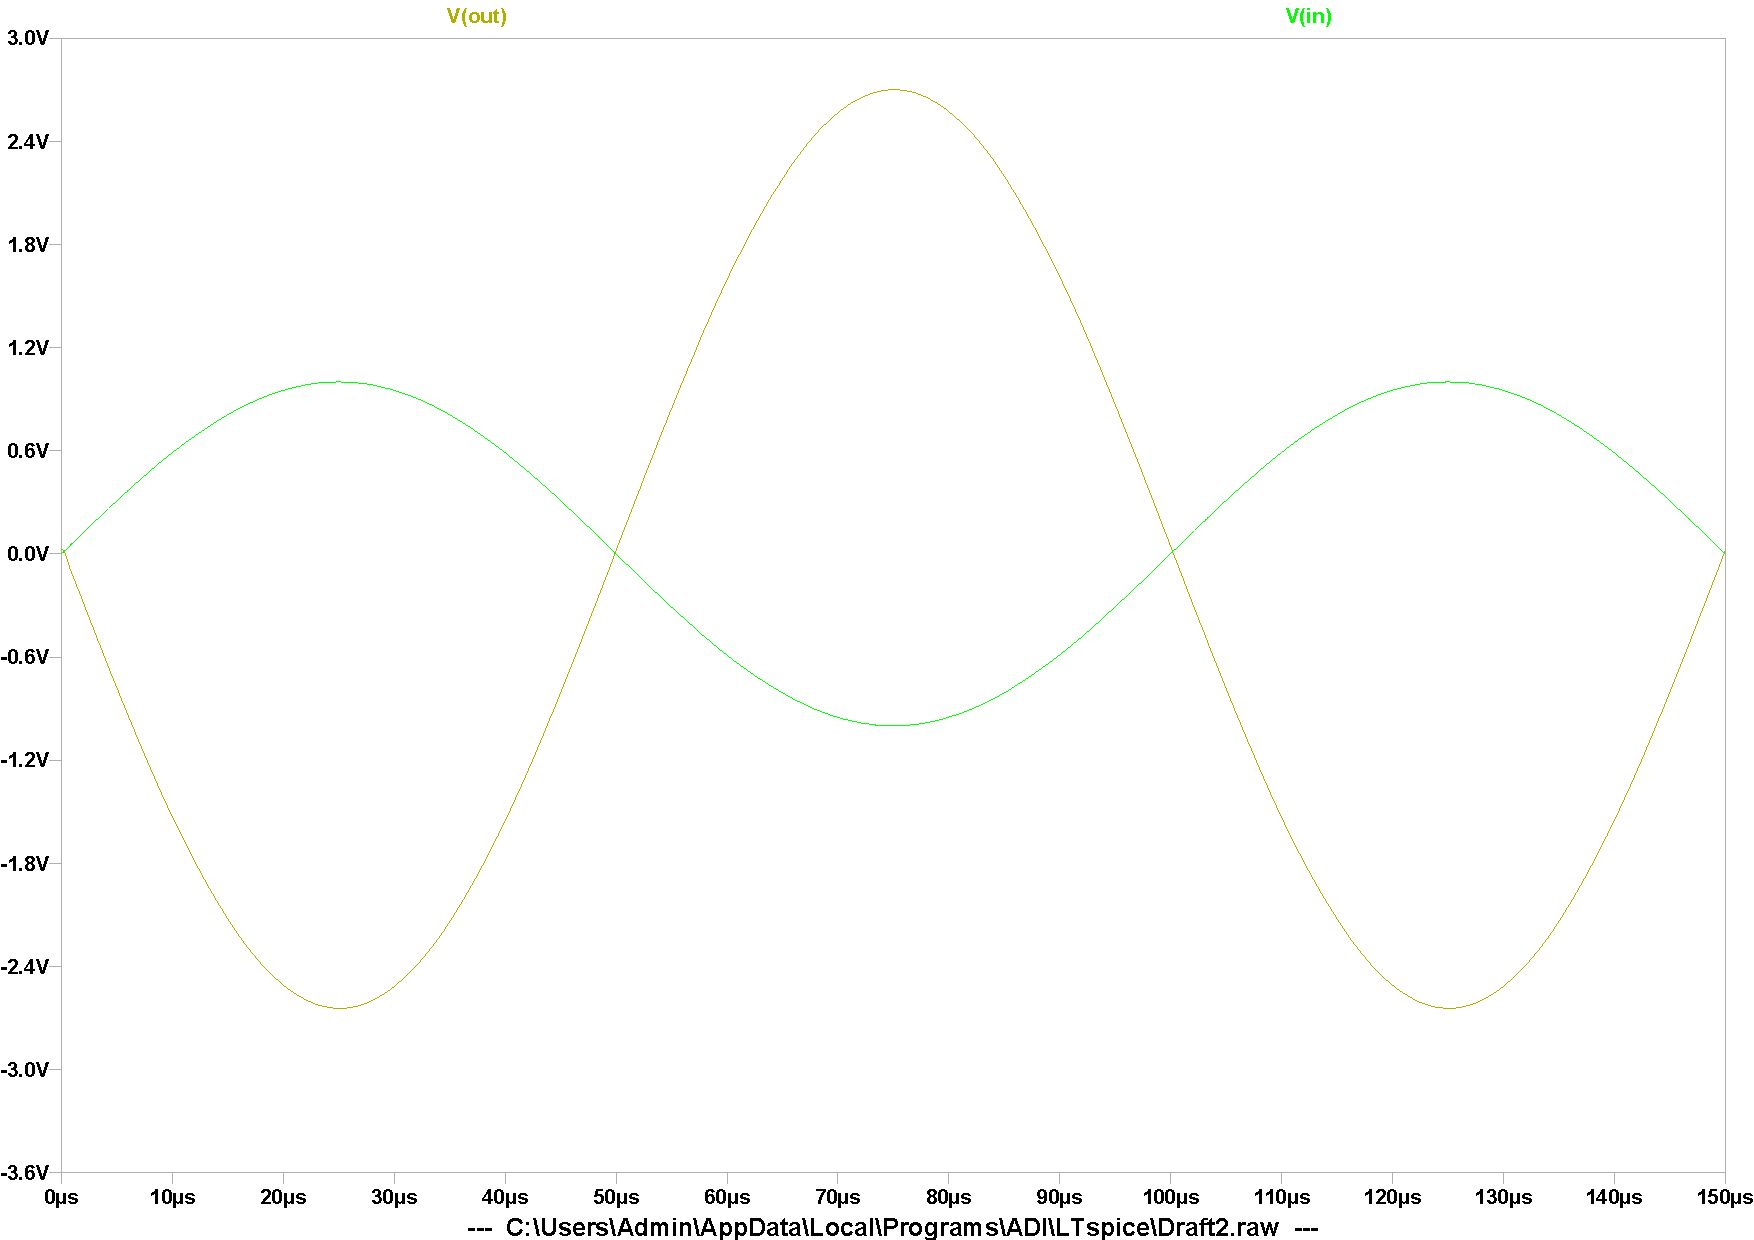
\includegraphics[width=\textwidth]{sim/bezporuch/tran.pdf}
  \caption{Simulace zapojení bez poruchy}
  \label{tran-bezPoruch}
\end{figure}

% --------------------------------------------------------------------------------- porucha 2

\begin{figure}[H]
  \centering
  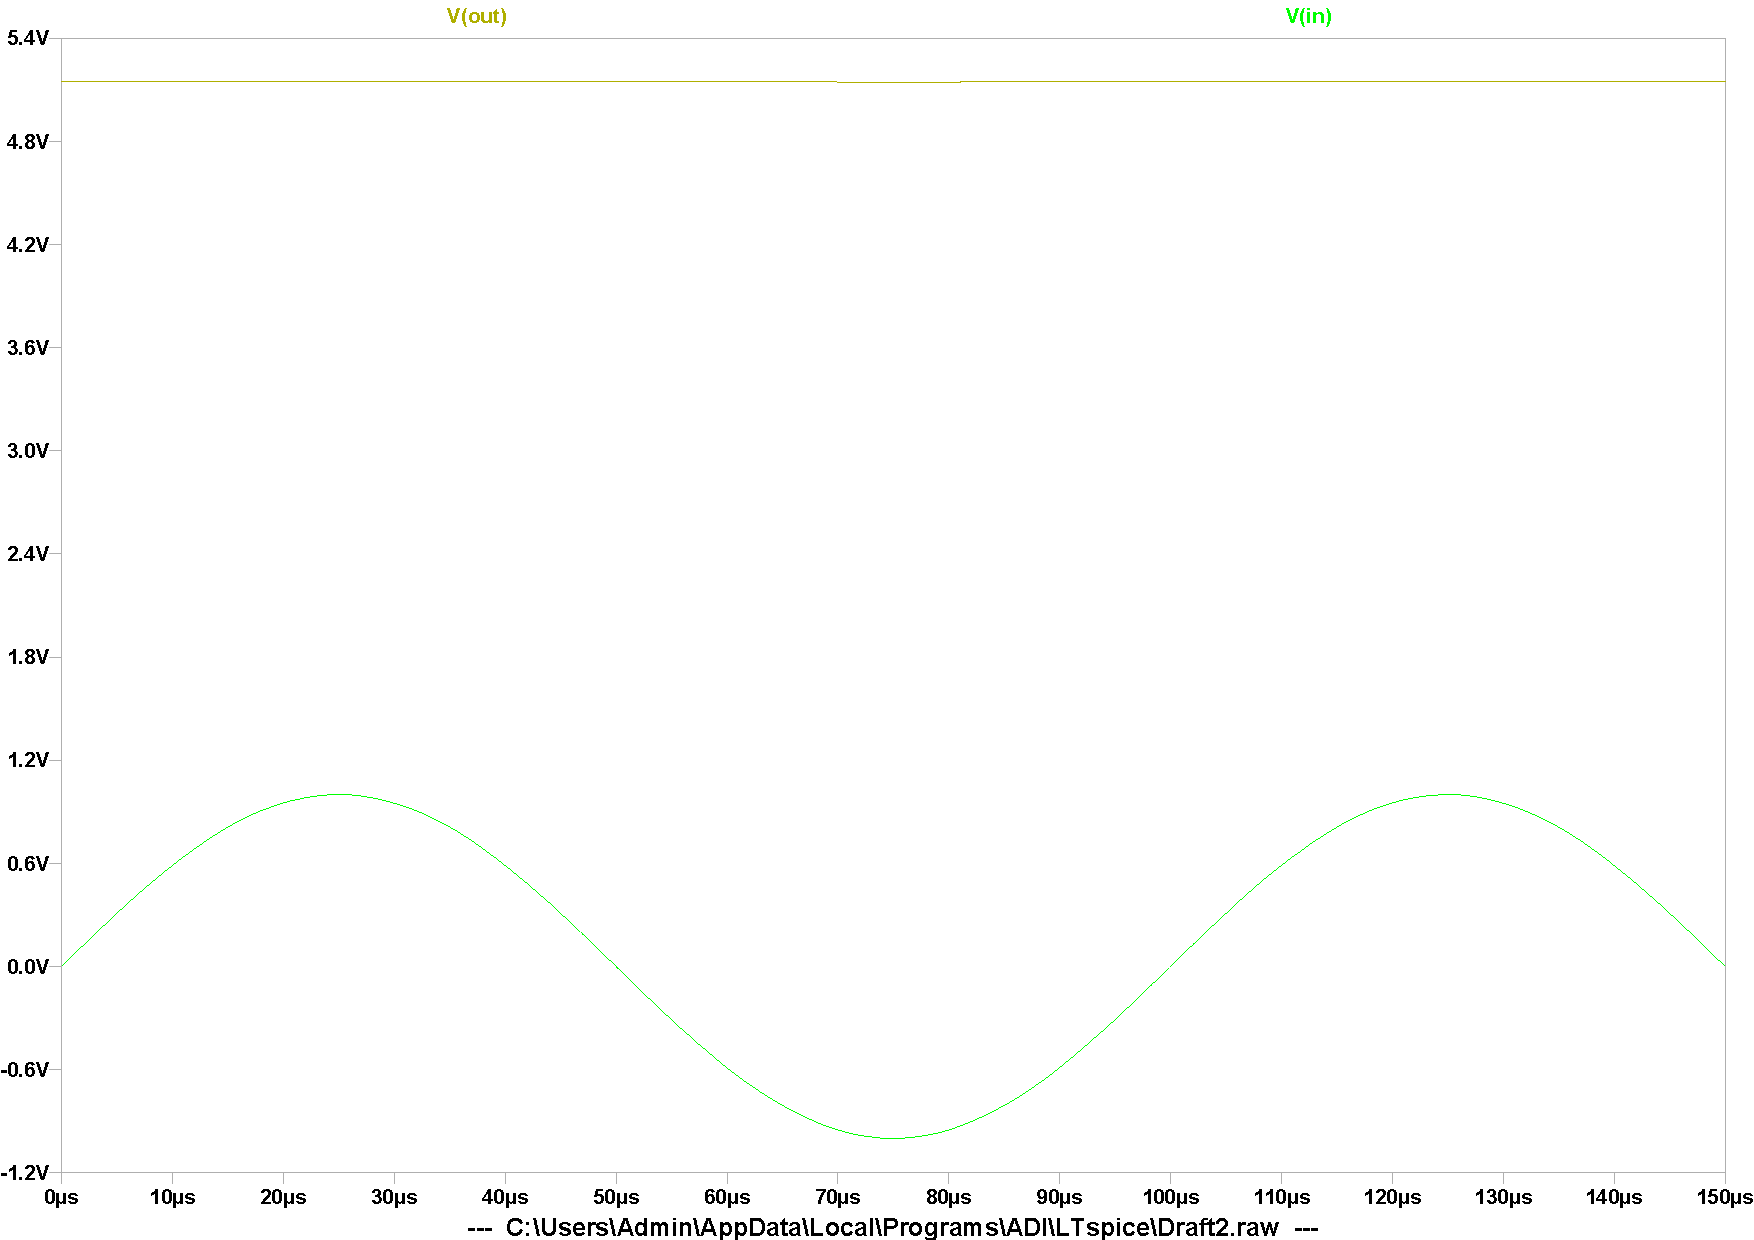
\includegraphics[width=0.95\textwidth]{sim/porucha-2/tran.pdf}
  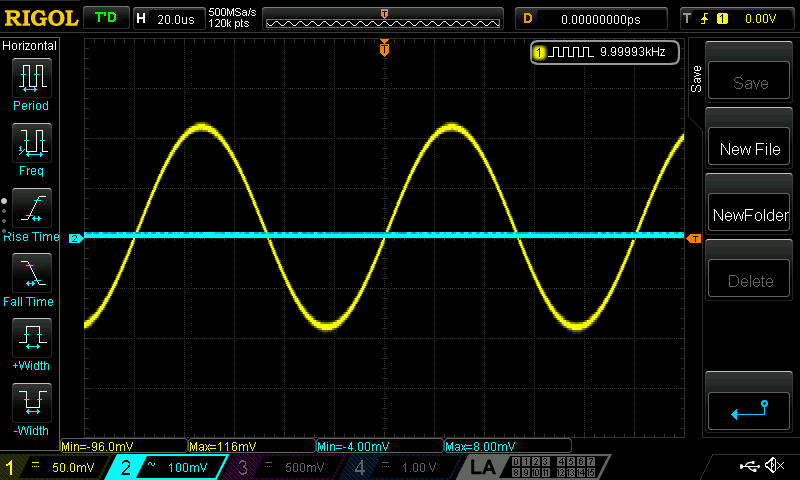
\includegraphics[width=0.9\textwidth]{mereni/NewFile3.png}
  \caption{Simulace a měření zkratu na odporu \(R_{Z2}\)}
  \label{tran-porucha2}
\end{figure}

% --------------------------------------------------------------------------------- porucha 3

\begin{figure}[H]
  \centering
  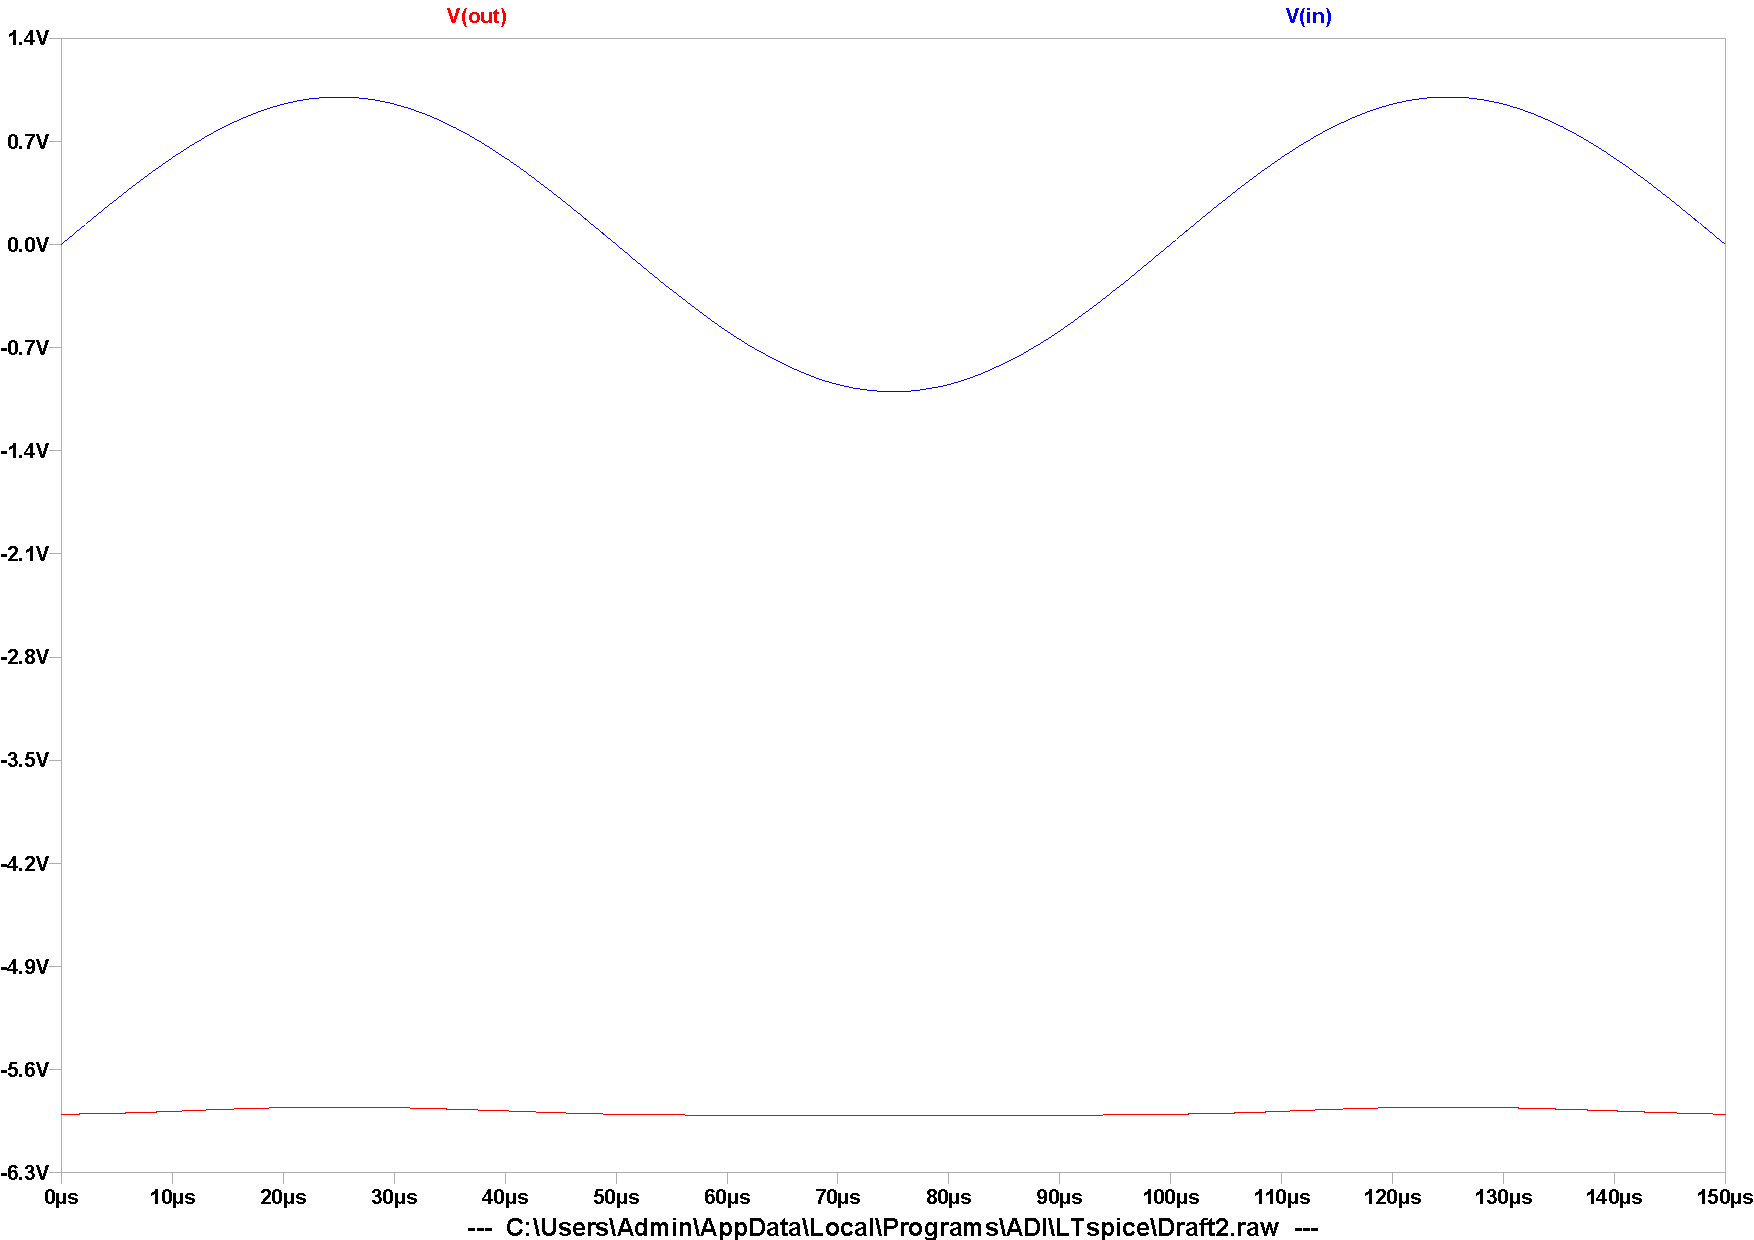
\includegraphics[width=\textwidth]{sim/porucha-3/tran.pdf}
  \caption{Simulace zkratu báze kolektor \(Q_5\)}
  \label{tran-porucha3}
\end{figure}

% --------------------------------------------------------------------------------- porucha 4

\begin{figure}[H]
  \centering
  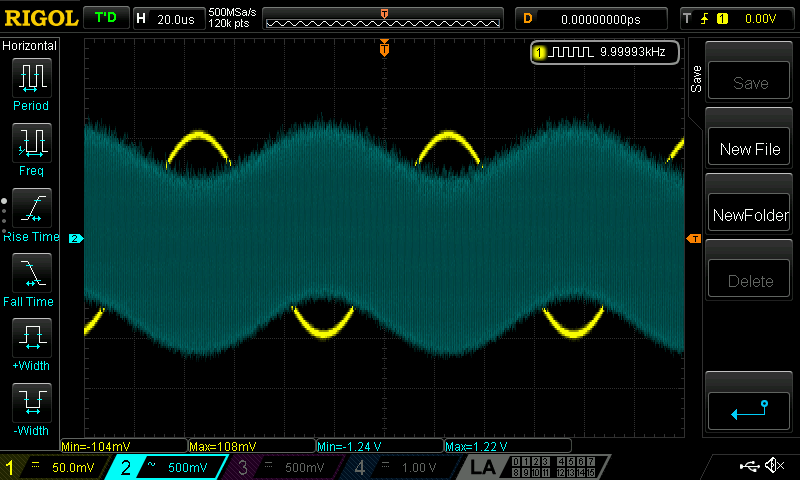
\includegraphics[width=\textwidth]{mereni/NewFile5.png}
  \caption{Měření rozpojení na \(C_1\)}
  \label{tran-porucha4}
\end{figure}

% --------------------------------------------------------------------------------- porucha 5

\begin{figure}[H]
  \centering
  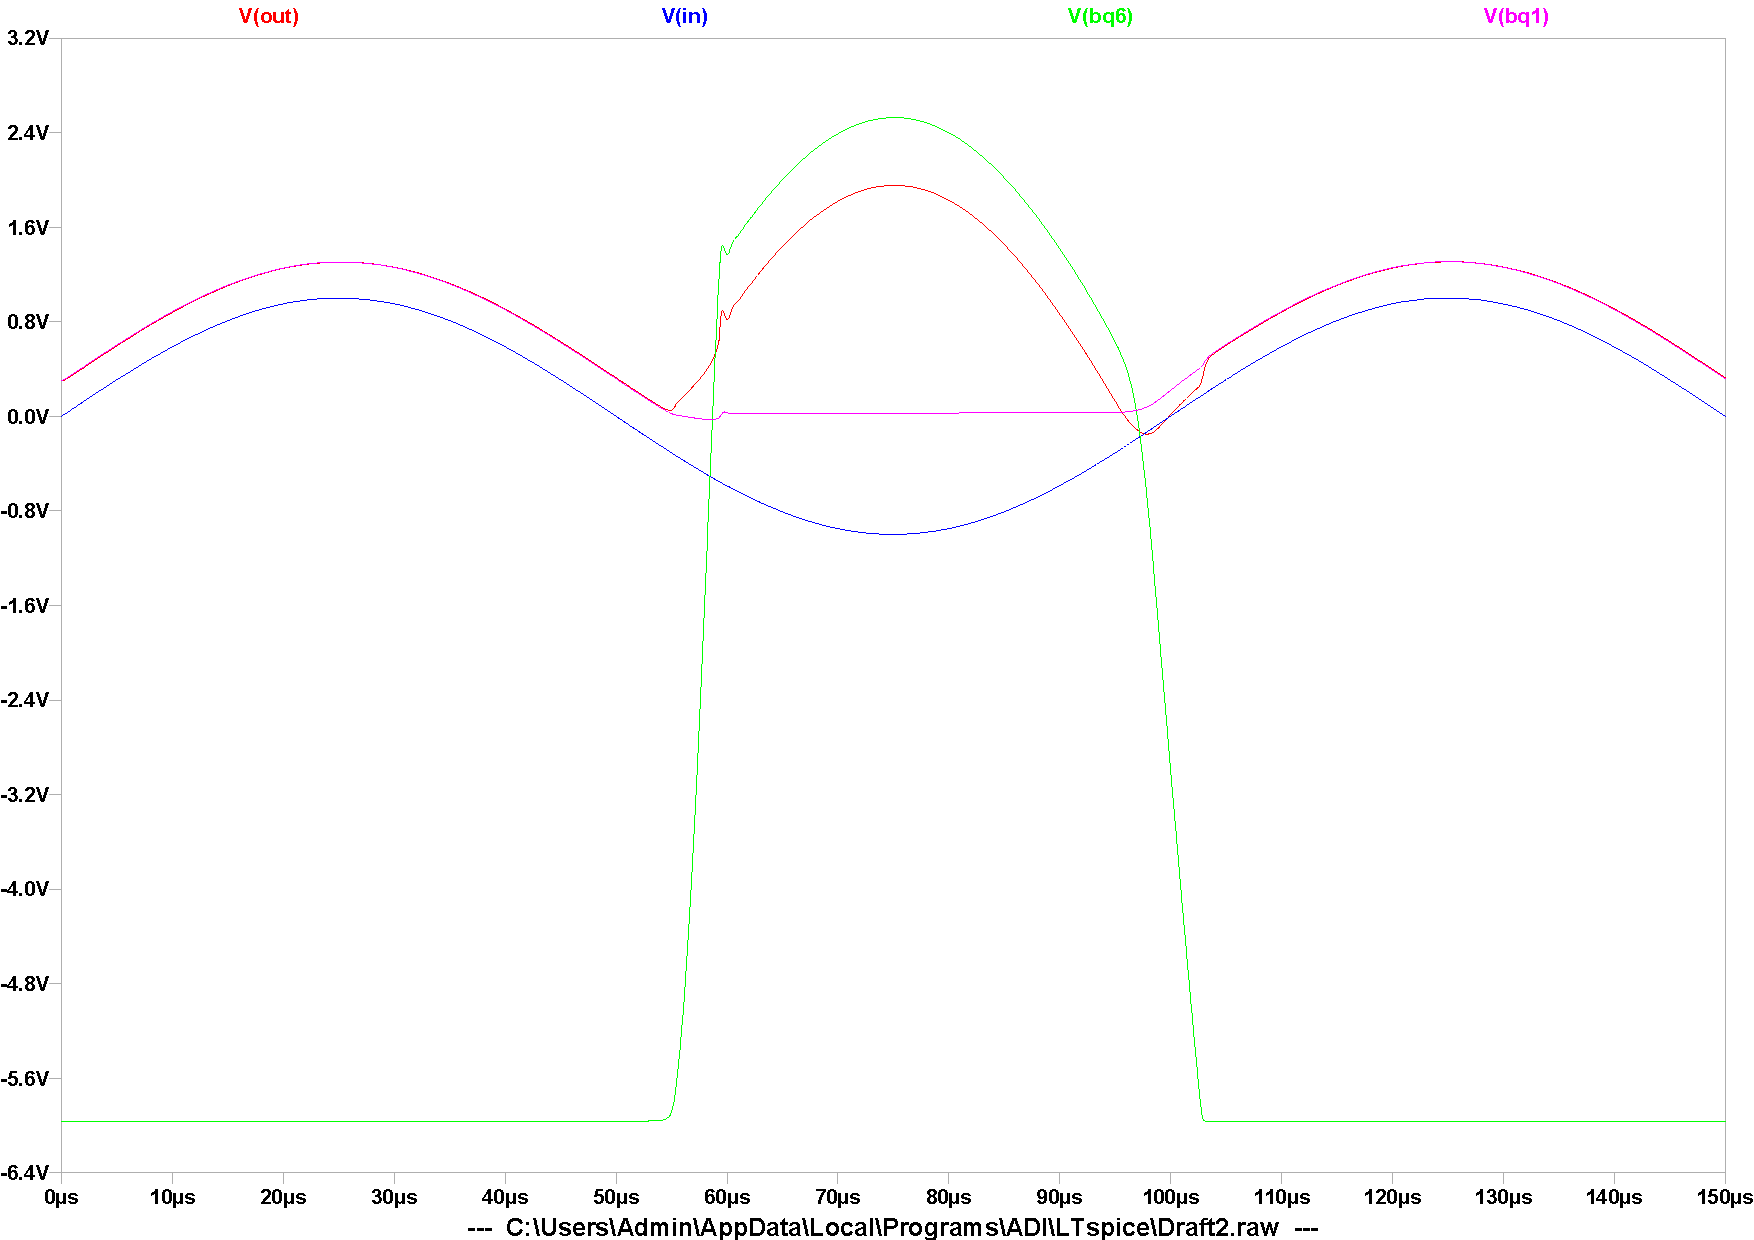
\includegraphics[width=\textwidth]{sim/porucha-5/tran.pdf}
  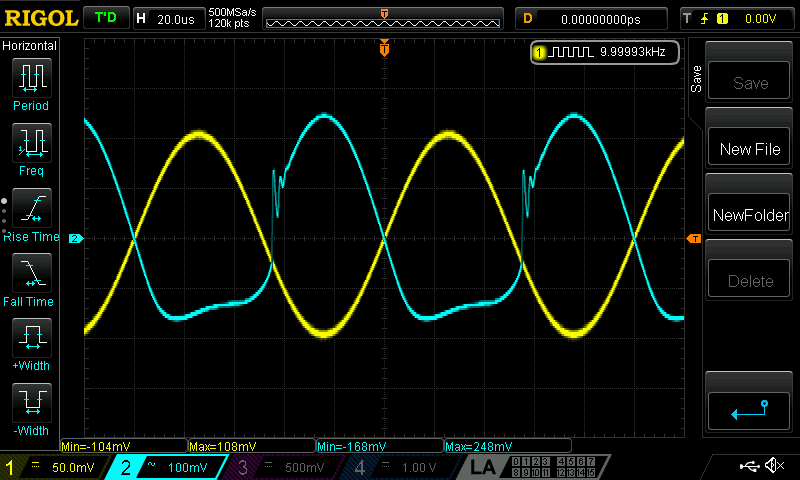
\includegraphics[width=0.95\textwidth]{mereni/NewFile9.png}
  \caption{Simulace a měření rozpojení na \(R_5\)}
  \label{tran-porucha5}
\end{figure}

\begin{figure}[H]
  \centering
  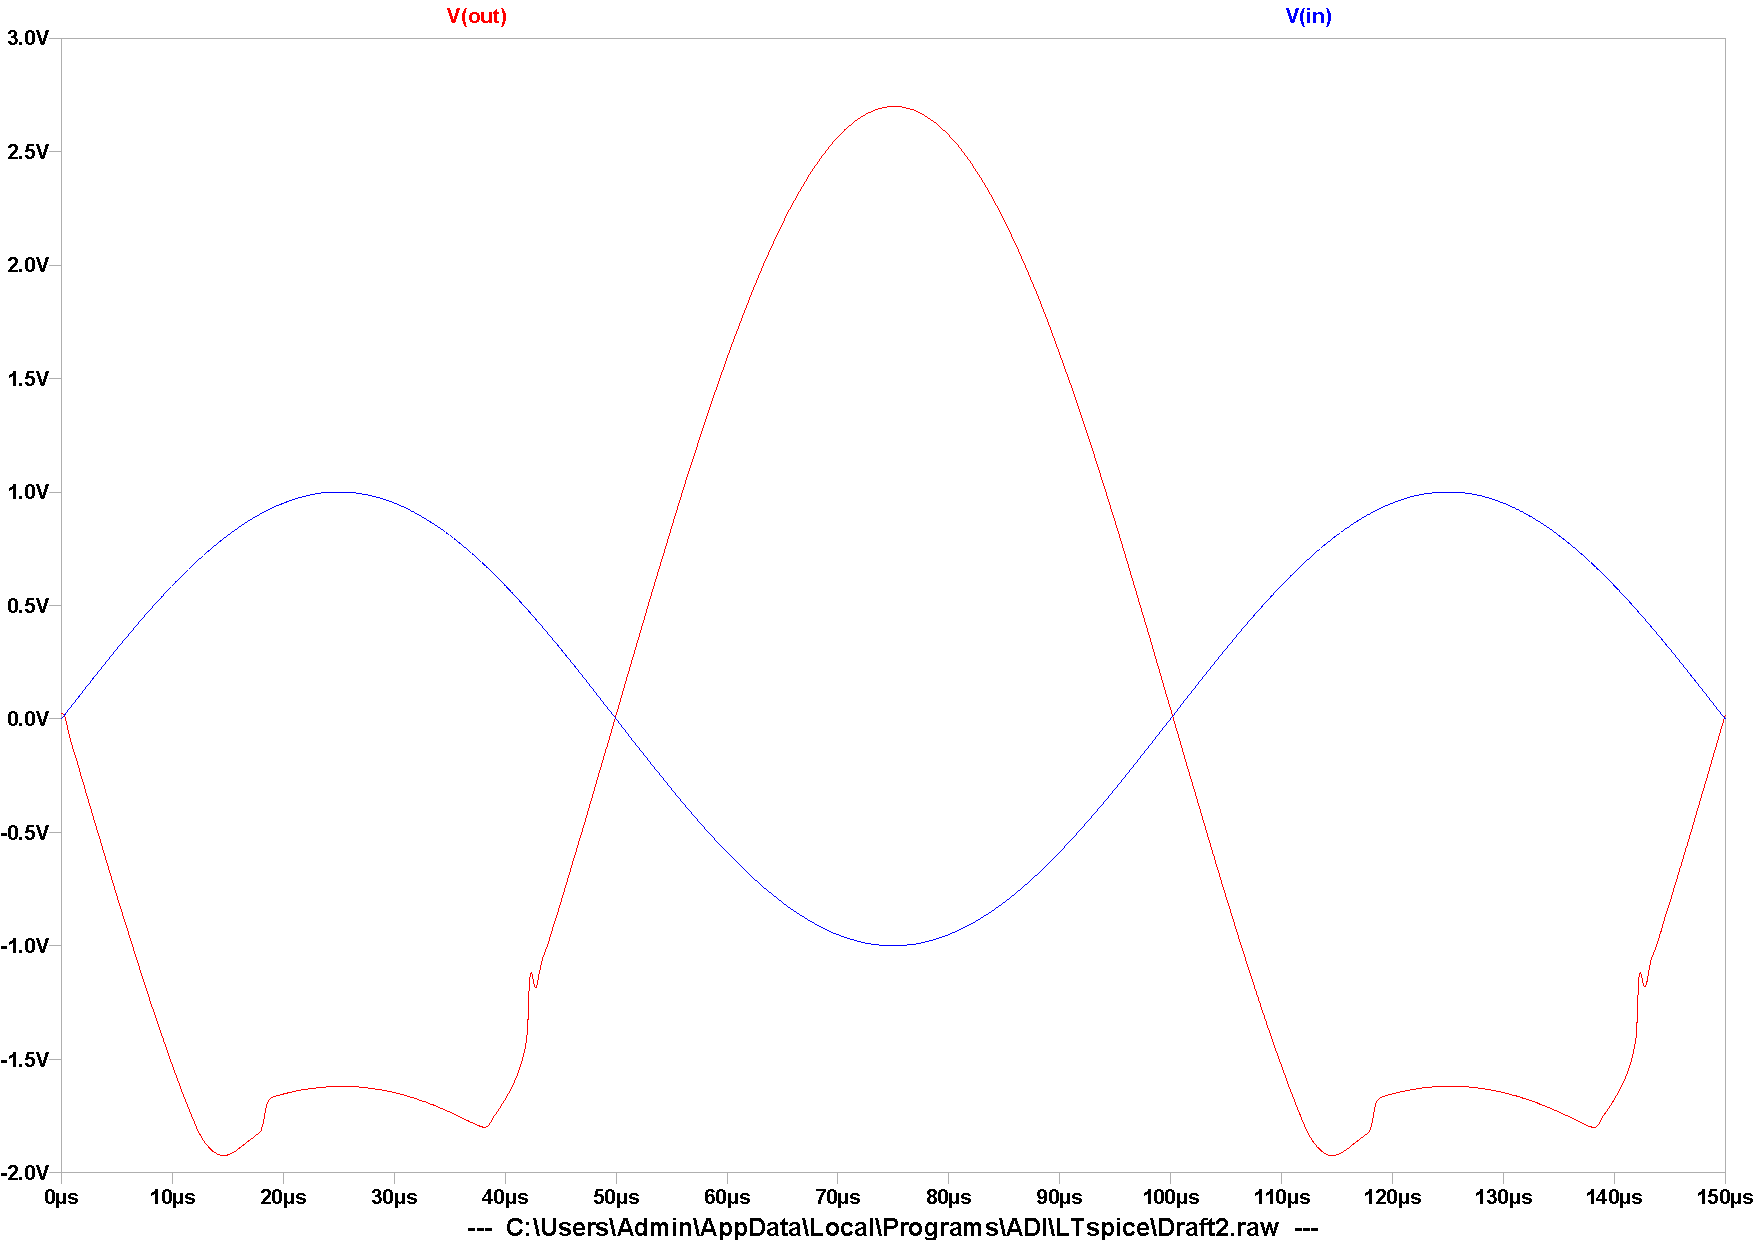
\includegraphics[width=\textwidth]{sim/porucha-5/tran-neuplne-rozpojeni.pdf}
  \caption{Simulace neúplného rozpojení, \(R_5 = 50k\)}
  \label{tran-porucha5-neuplna}
\end{figure}


% --------------------------------------------------------------------------------- porucha 6

\begin{figure}[H]
  \centering
  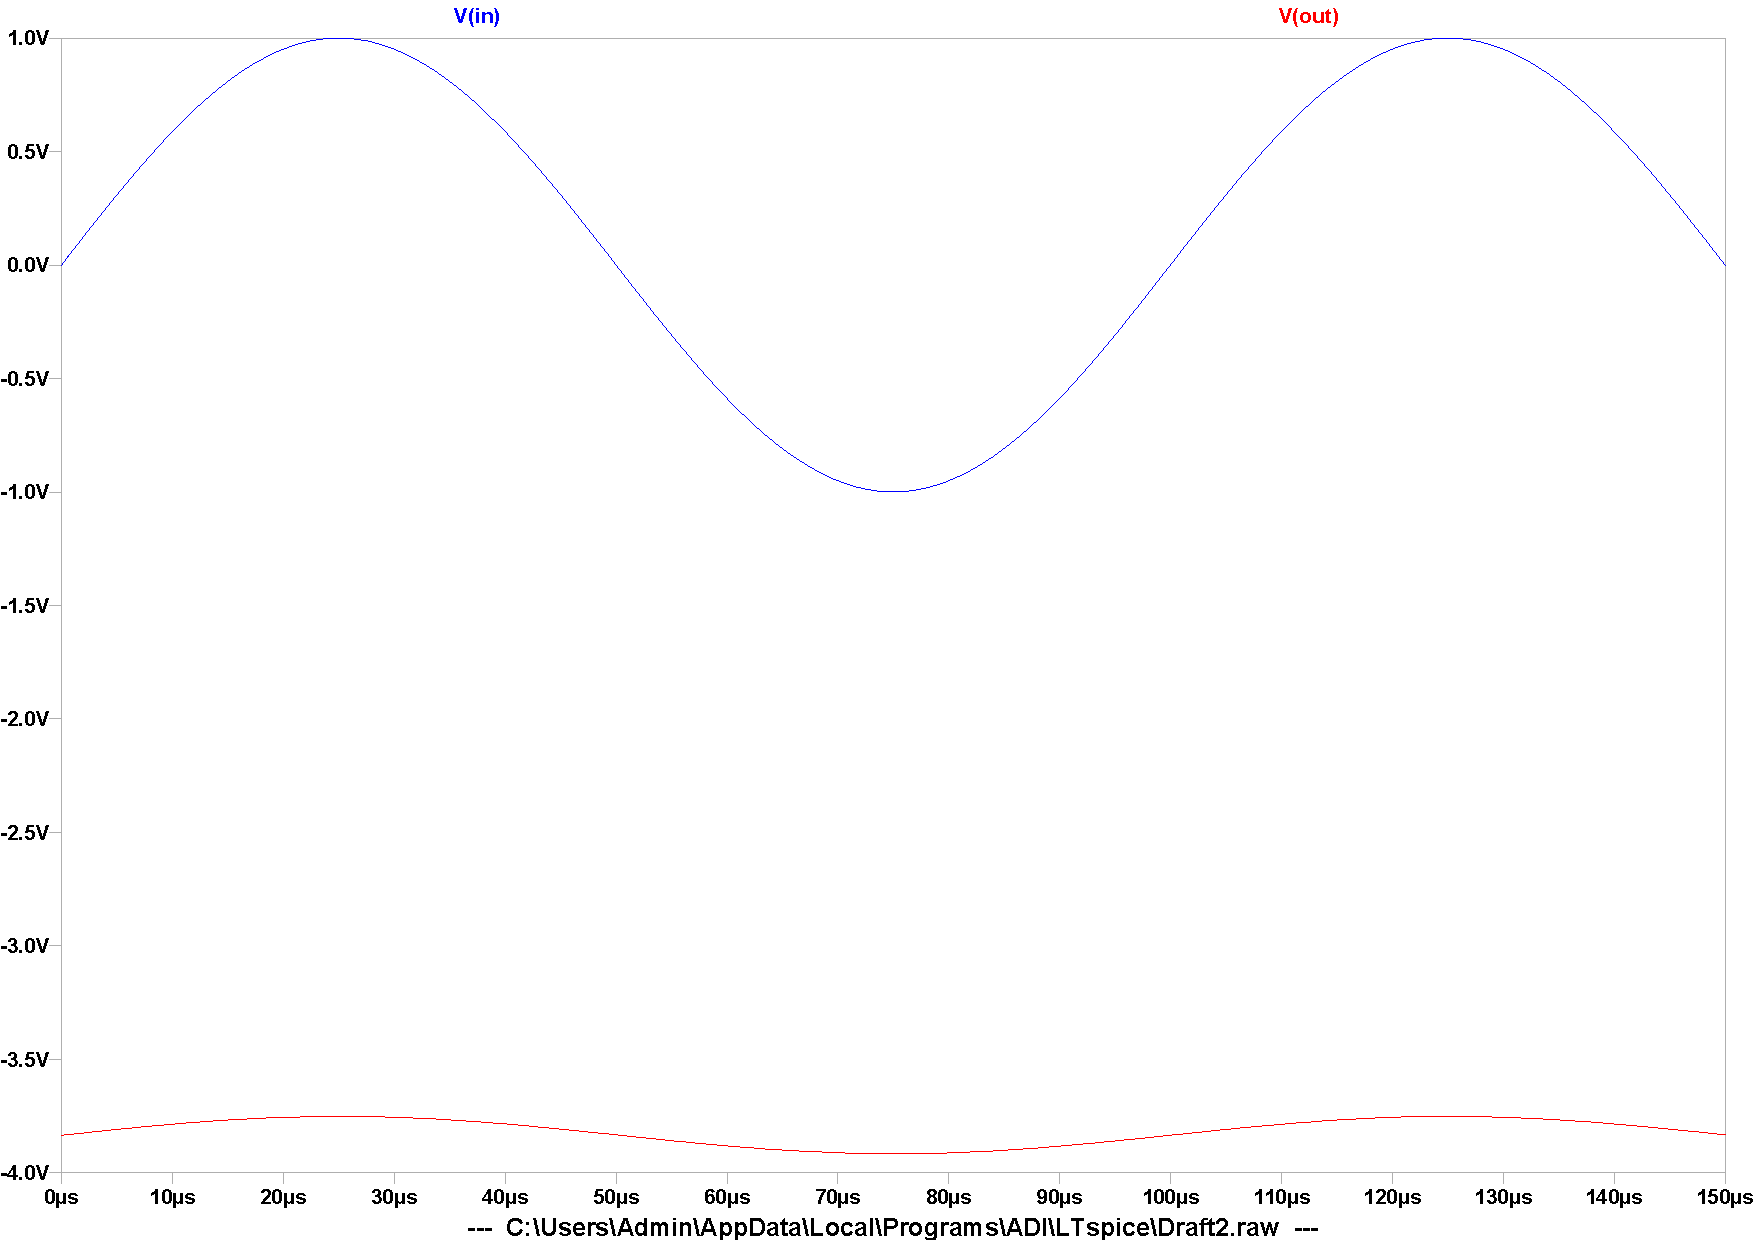
\includegraphics[width=\textwidth]{sim/porucha-6/tran.pdf}
  \caption{Simulace zkratu mezi bází a emitorem \(Q_6\)}
  \label{tran-porucha6}
\end{figure}

% --------------------------------------------------------------------------------- porucha 7

\begin{figure}[H]
  \centering
  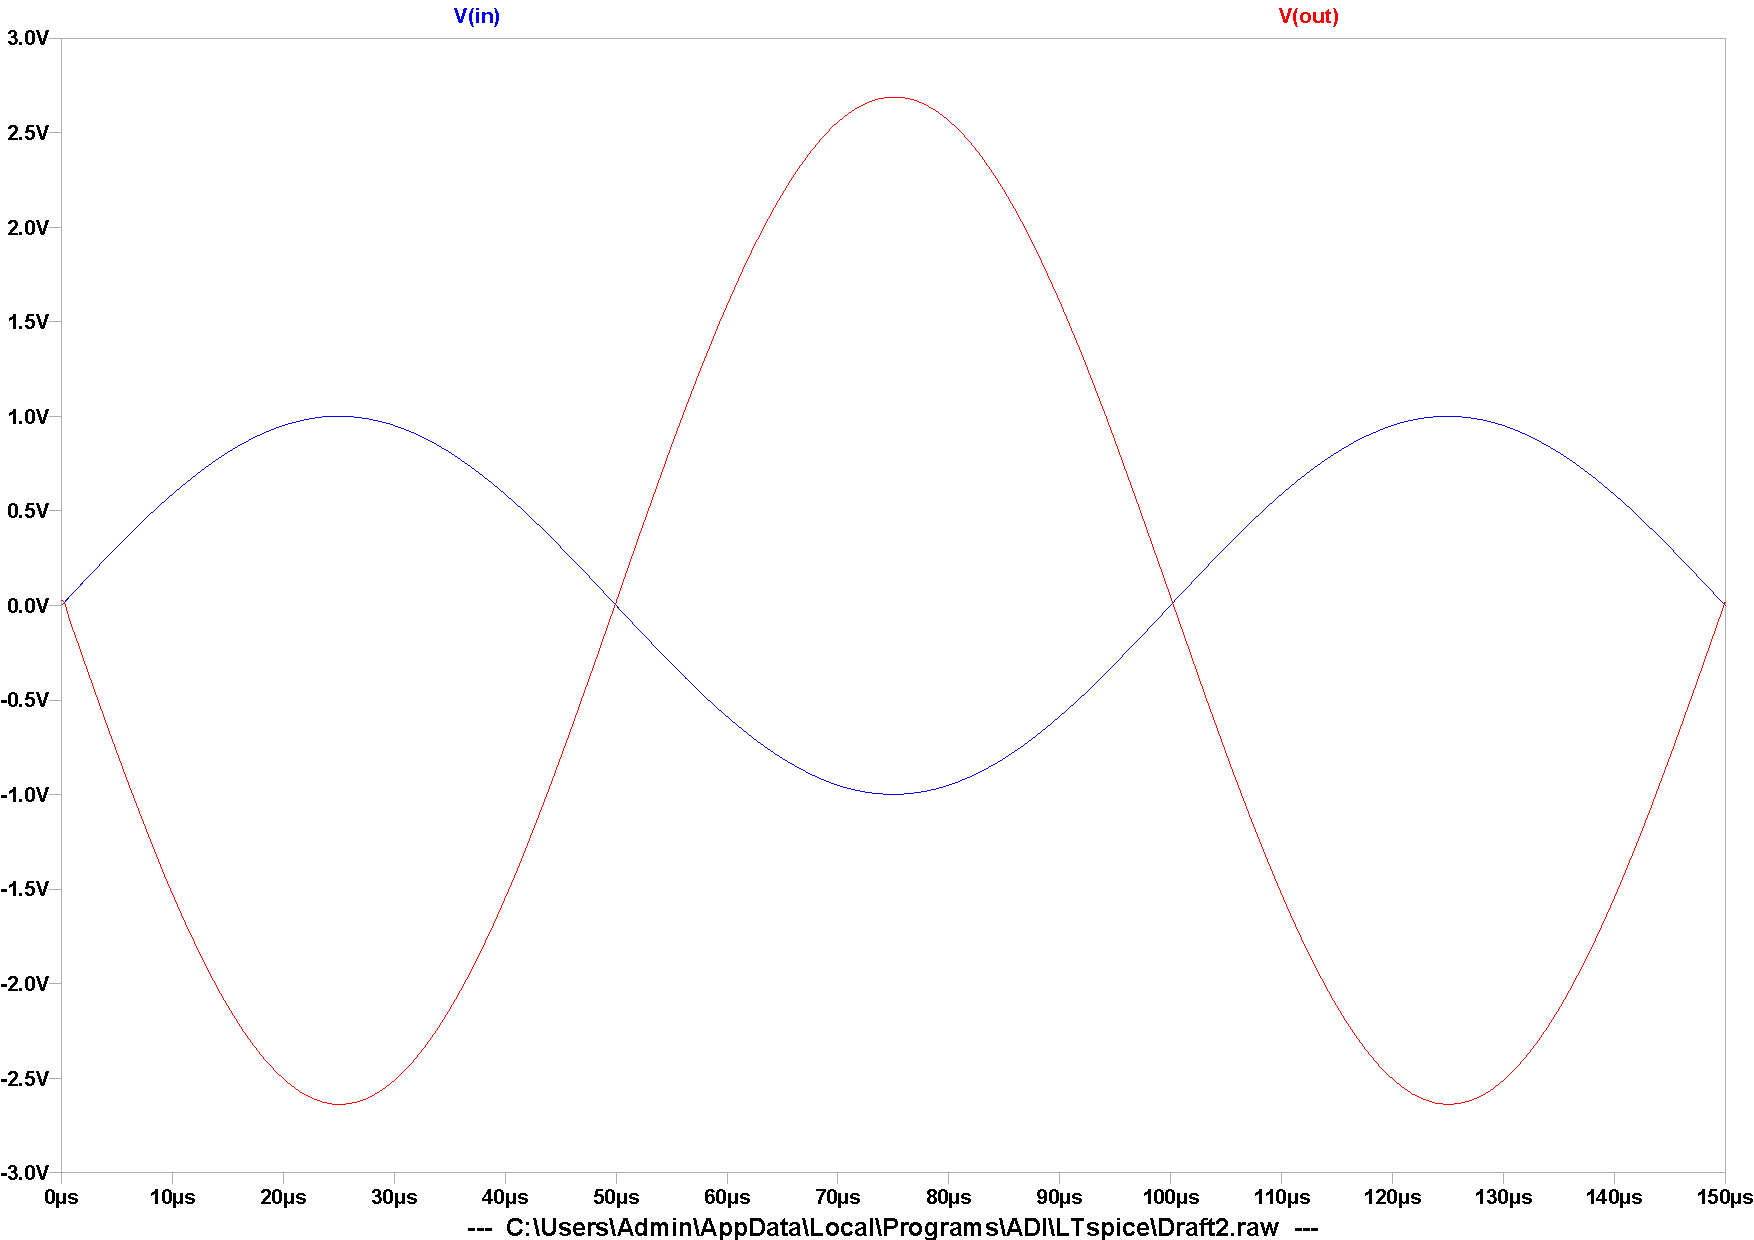
\includegraphics[width=\textwidth]{sim/porucha-7/tran.pdf}
  \caption{Simulace zkratu mezi bází a emitorem \(Q_6\) a rozpojení na \(R_5\)}
  \label{tran-porucha6}
\end{figure}


% Zesilovač má zesílením lehce menší \(1\), což je vidět na simulovaném průběhu bez poruch \obr{fig:sch-sc-bezPoruch} i na měřeném průběhu.

% Při rozpojení na \(R_2\) neboli \(R_{B2}\) se posouvají mezní napětí a saturace v záporné půlvlně tak nastává mnohem dřív než v kladné půlvlně.
% Simulace viz \obr{fig:sch-sc-p2}.
% Až na stejnosměrný posun se simulace a měření shodují.

% Při rozpojení na \(R_3\) neboli \(R_E\) zásadně vzrůstá výstupní odpor a výstup proto nemůžeme zatížit bez zkreslení.
% V simulaci \obr{fig:sch-sc-p3} je proto použit odpor \(R_4 = 100\-[k]\), aby se vysoký výstupní odpor projevil.
% Měření ukazuje trochu jinak zkreslený signál, jinak ale simulace odpovídá.


% Zkrat mezi bází a kolektorem má za následek trvalé otevření tranzistoru a na výstup se tak vstupní napětí nemá jak dostat. 
% Simulace viz \obr{fig:sch-sc-p4}.
% Simulace a měření se shodují.


% Zkrat mezi bází a emitorem má za následek růst výstupního odporu, neboli vyřazení proudového zesílení zesilovače.
% Simulace viz \obr{fig:sch-sc-p5}


% Zkrat mezi kolektorem a emitorem vyřazuje tranzistor z provozu a na výstup se tak napětí ze vstupu nedostává.
% Simulace viz \obr{fig:sch-sc-p6}


% \begin{figure}[H]
%   \centering
%   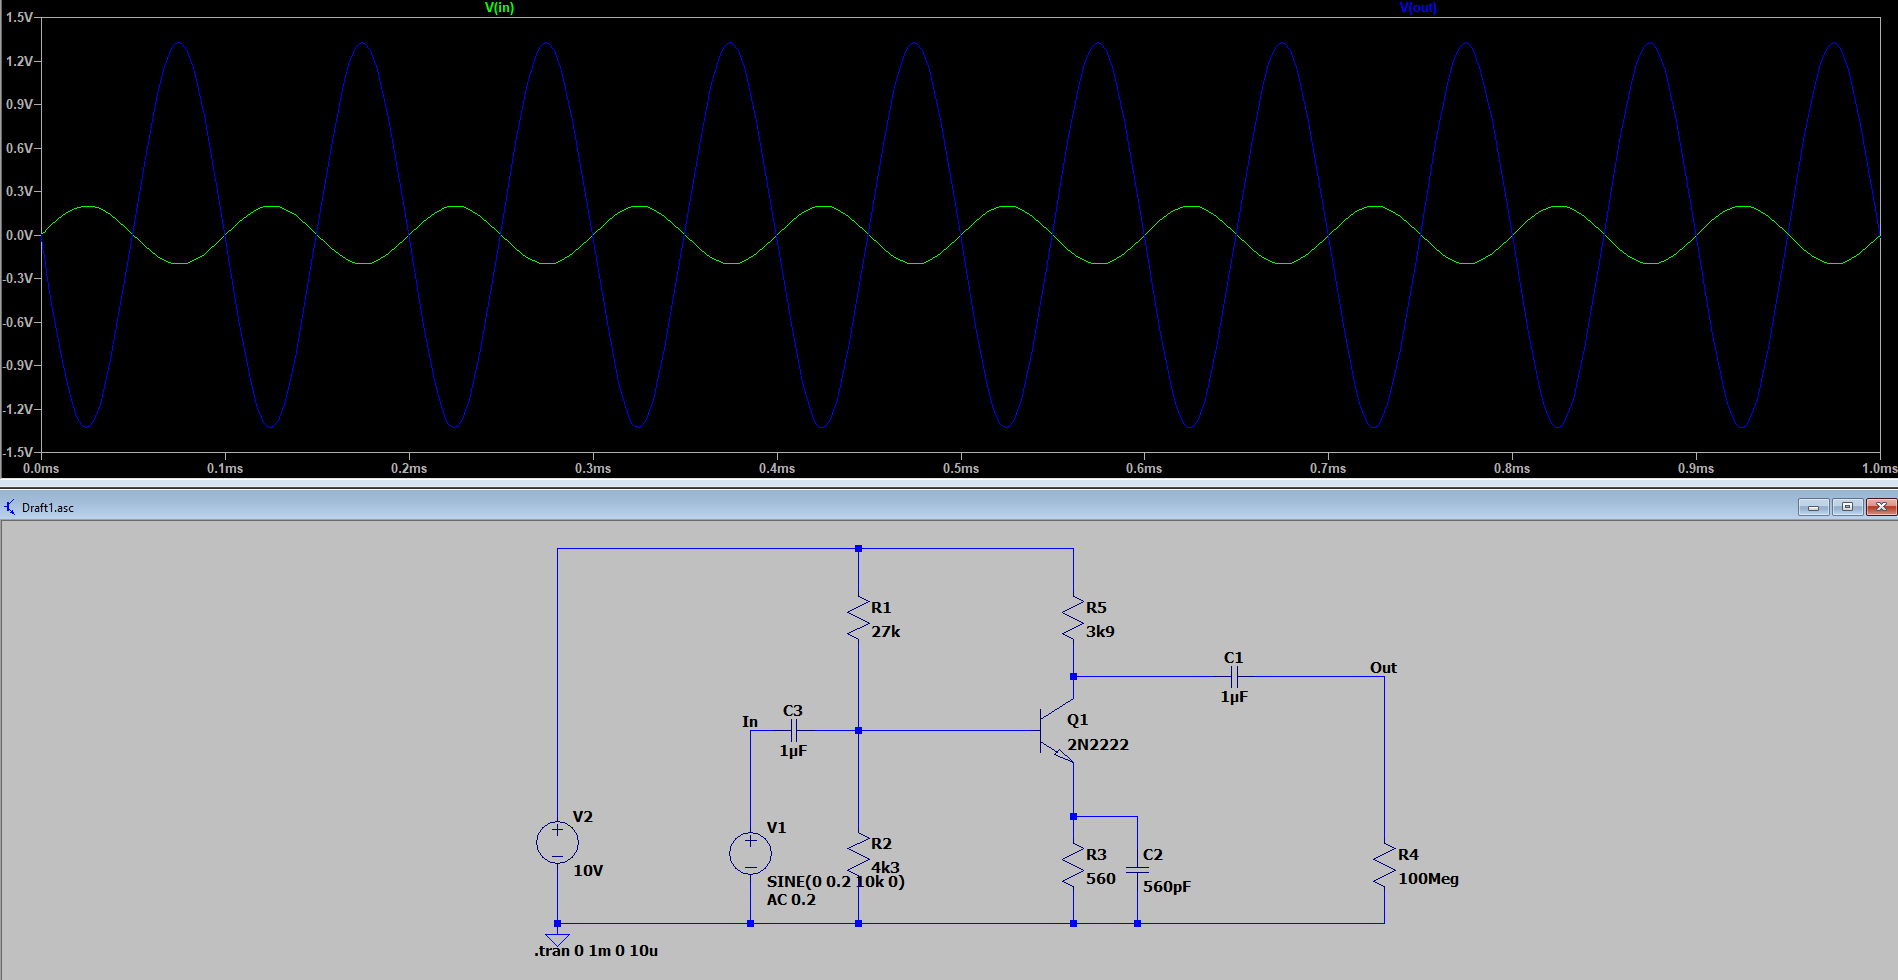
\includegraphics[width=\textwidth]{sim/ukol2/bezPoruch.png}
%   \caption{Simulace zapojení bez poruchy}
%   \label{fig:sch-sc-bezPoruch}
% \end{figure}

% \begin{figure}[H]
%   \centering
%   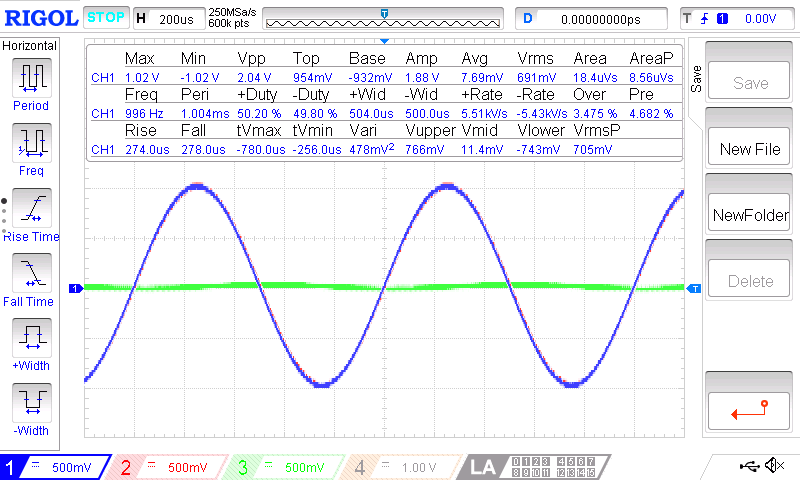
\includegraphics[width=0.95\textwidth]{mereni/NewFolder1/NewFile8.png}
%   \caption{Měření zapojení bez poruchy}
%   \label{fig:m-sch-sc-bezPoruch}
% \end{figure}

% % ---------------------------------------------------------------------------------

% \begin{figure}[H]
%   \centering
%   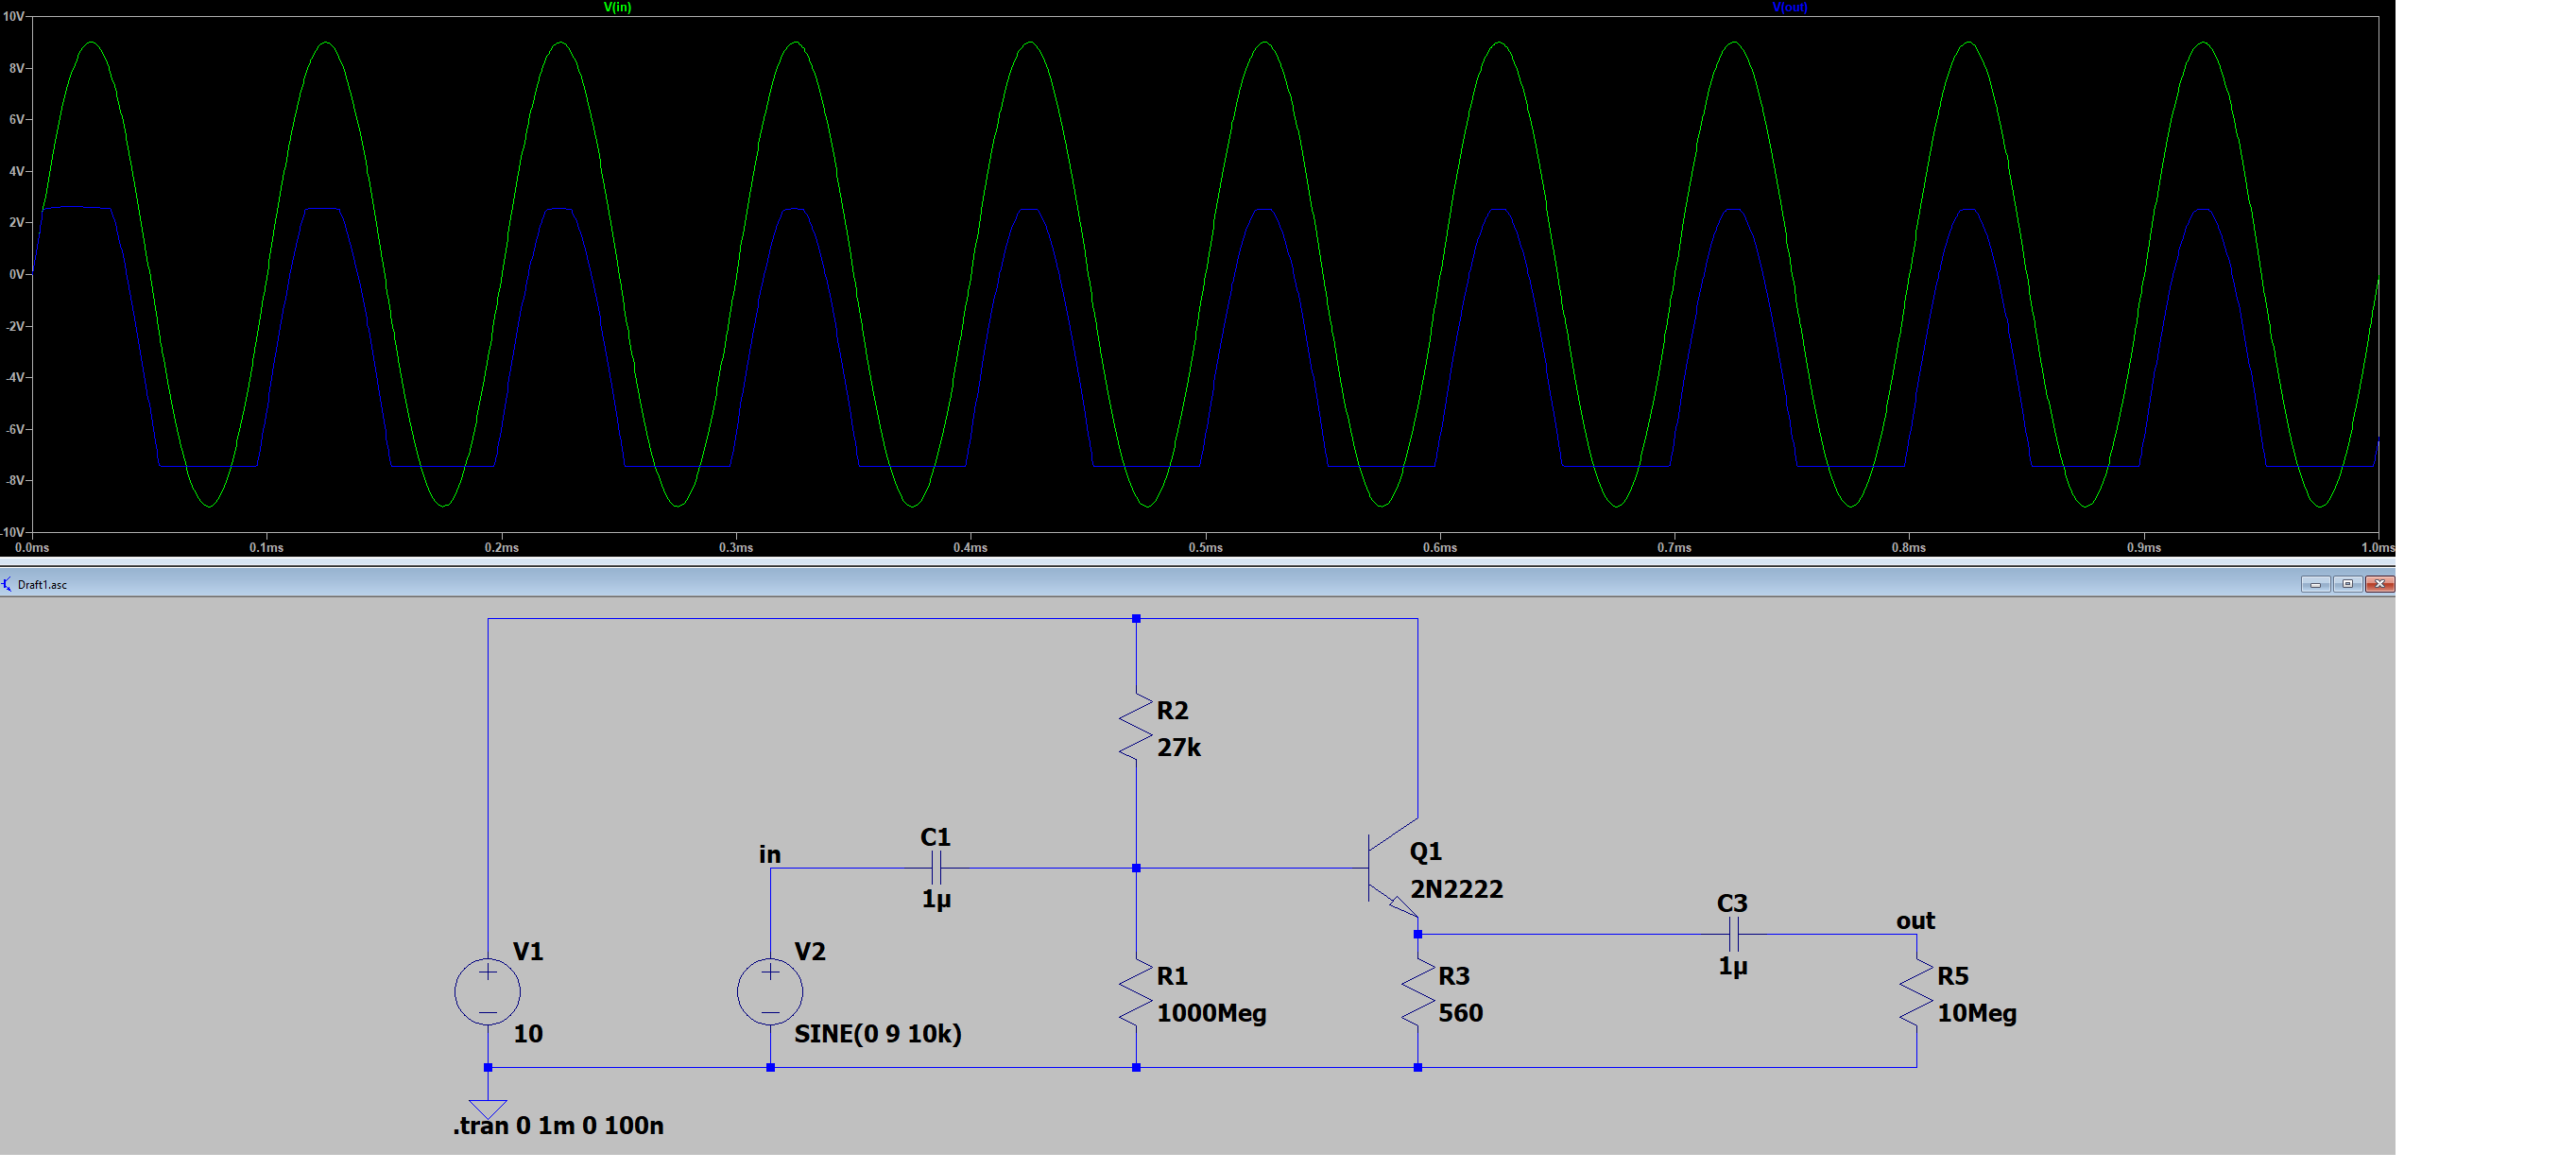
\includegraphics[width=\textwidth]{sim/ukol2/porucha1.png}
%   \caption{Simulace rozpojení na odporu \(R_2\) neboli \(R_{B2}\)}
%   \label{fig:sch-sc-p2}
% \end{figure}

% \begin{figure}[H]
%   \centering
%   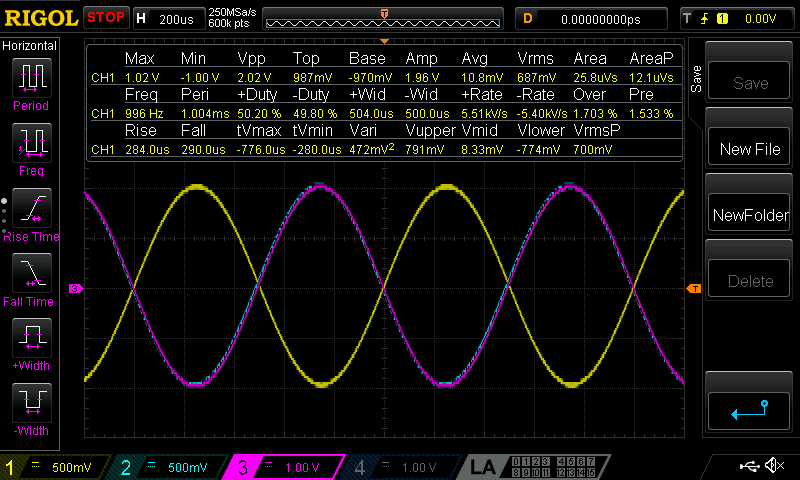
\includegraphics[width=0.95\textwidth]{mereni/NewFolder1/NewFile9.png}
%   \caption{Měření rozpojení na odporu \(R_2\) neboli \(R_{B2}\)}
%   \label{fig:m-sch-sc-p2}
% \end{figure}

% % ---------------------------------------------------------------------------------

% \begin{figure}[H]
%   \centering
%   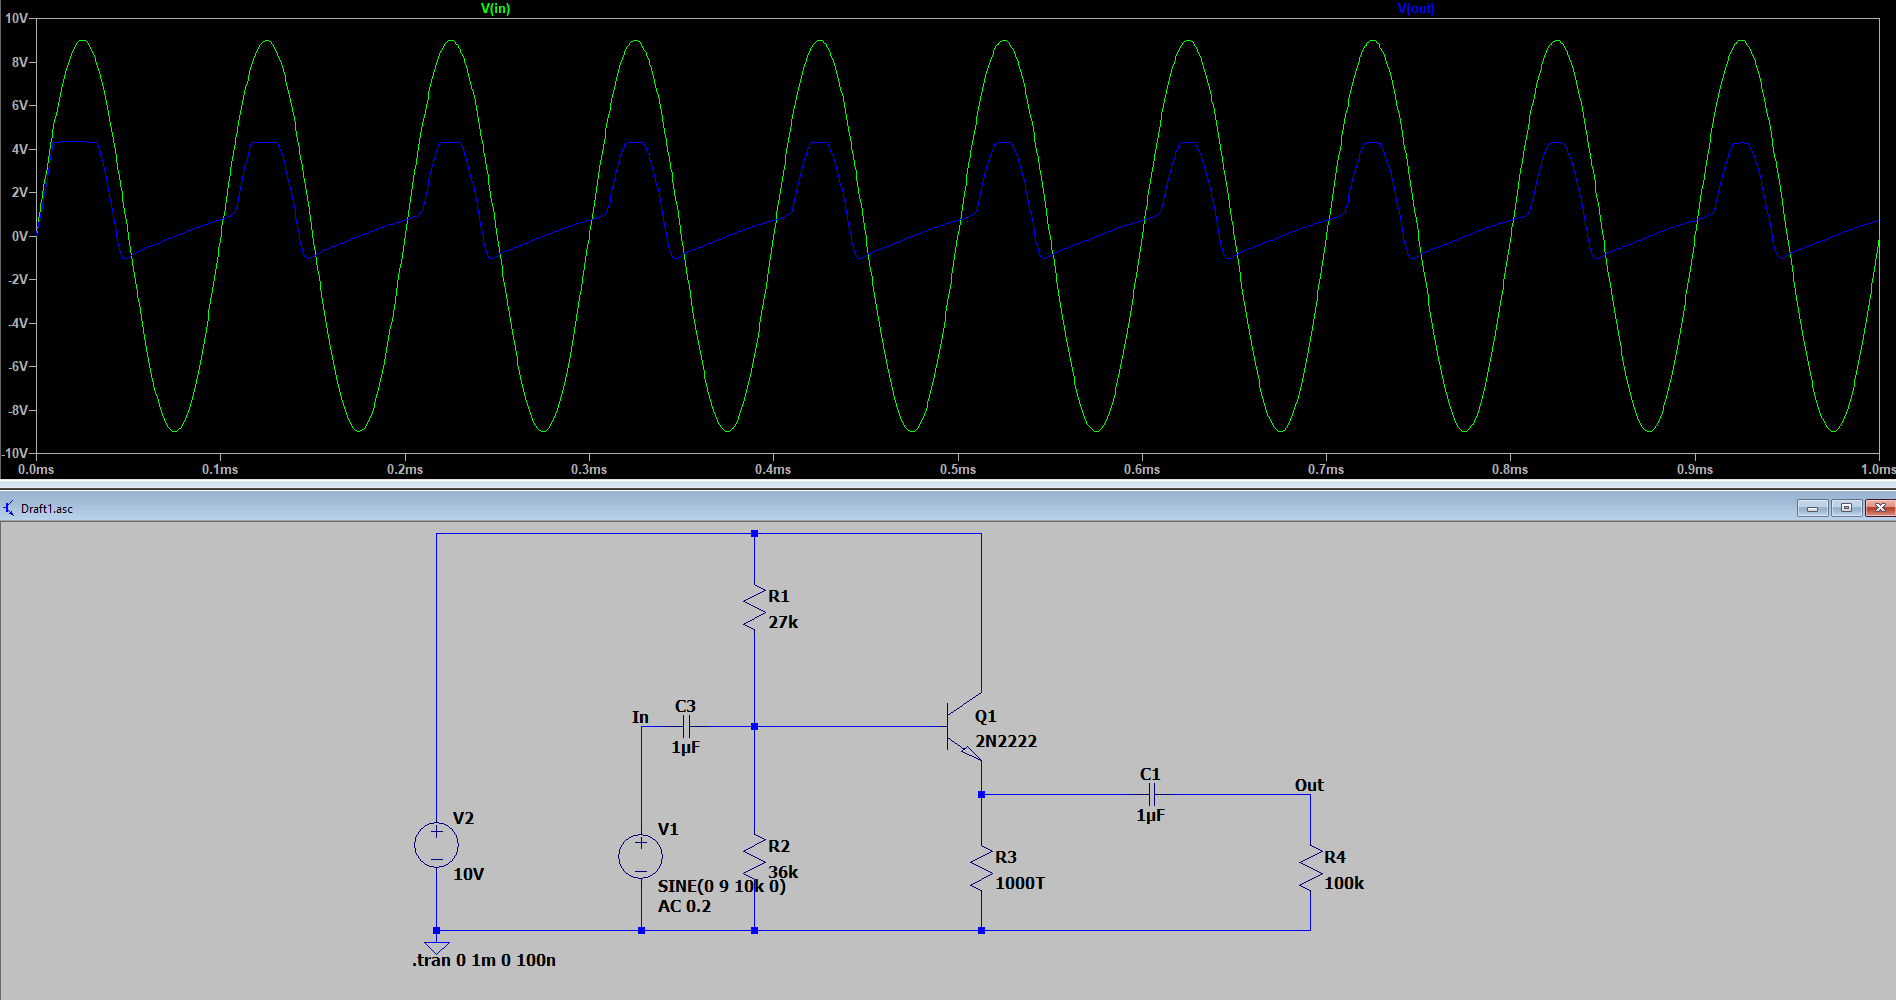
\includegraphics[width=\textwidth]{sim/ukol2/porucha2-seZatezi100k.png}
%   \caption{Simulace rozpojení na odporu \(R_3\) neboli \(R_{E}\)}
%   \label{fig:sch-sc-p3}
% \end{figure}

% \begin{figure}[H]
%   \centering
%   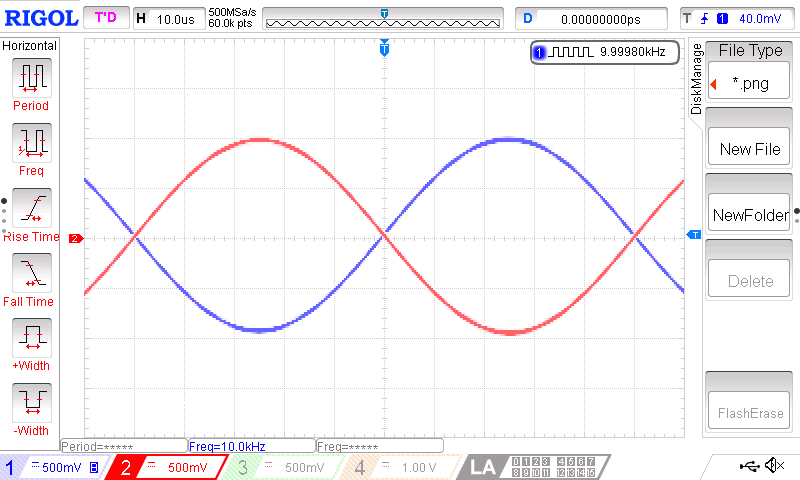
\includegraphics[width=0.95\textwidth]{mereni/NewFolder1/NewFile10.png}
%   \caption{Měření rozpojení na odporu \(R_3\) neboli \(R_{E}\)}
%   \label{fig:m-sch-sc-p3}
% \end{figure}

% % ---------------------------------------------------------------------------------

% \begin{figure}[H]
%   \centering
%   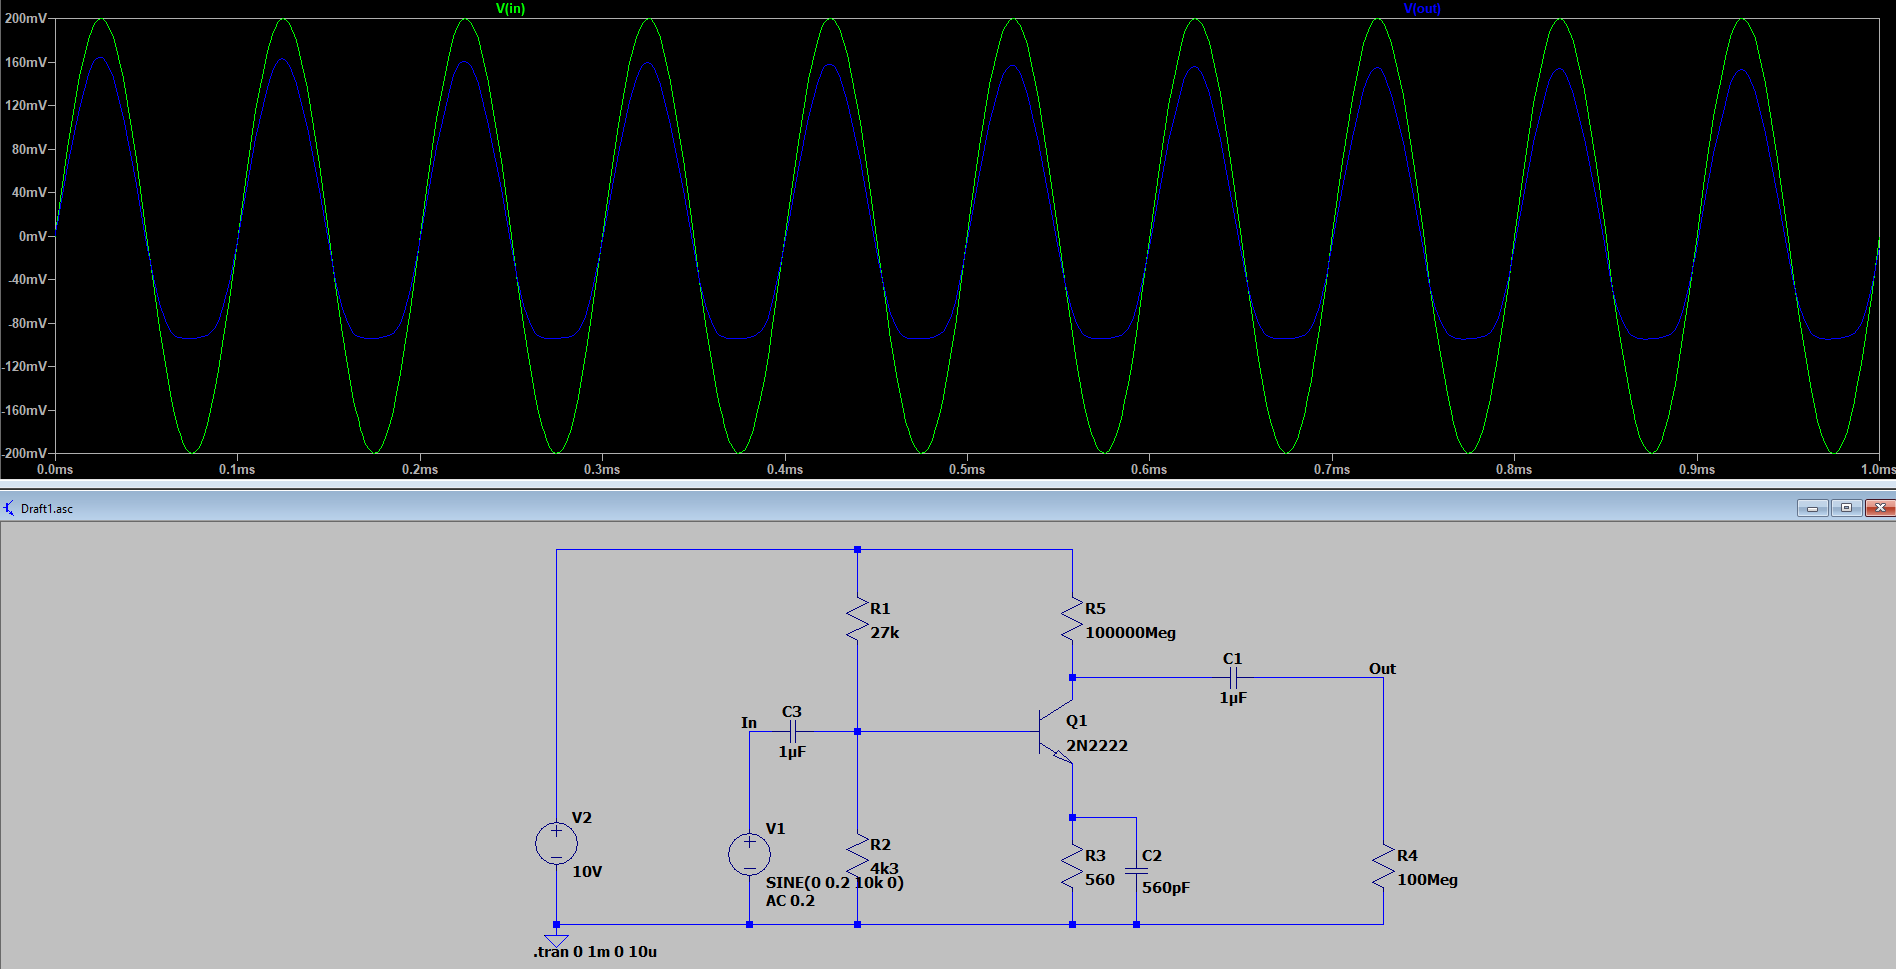
\includegraphics[width=\textwidth]{sim/ukol2/porucha3.png}
%   \caption{Simulace zkratu mezi bází a kolektorem}
%   \label{fig:sch-sc-p4}
% \end{figure}

% \begin{figure}[H]
%   \centering
%   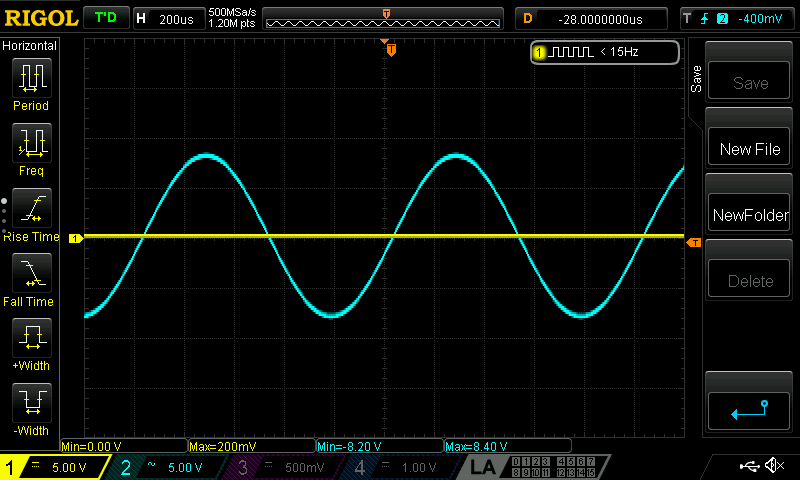
\includegraphics[width=0.95\textwidth]{mereni/NewFolder1/NewFile13.png}
%   \caption{Měření zkratu mezi bází a kolektorem}
%   \label{fig:m-sch-sc-p4}
% \end{figure}

% % ---------------------------------------------------------------------------------

% \begin{figure}[H]
%   \centering
%   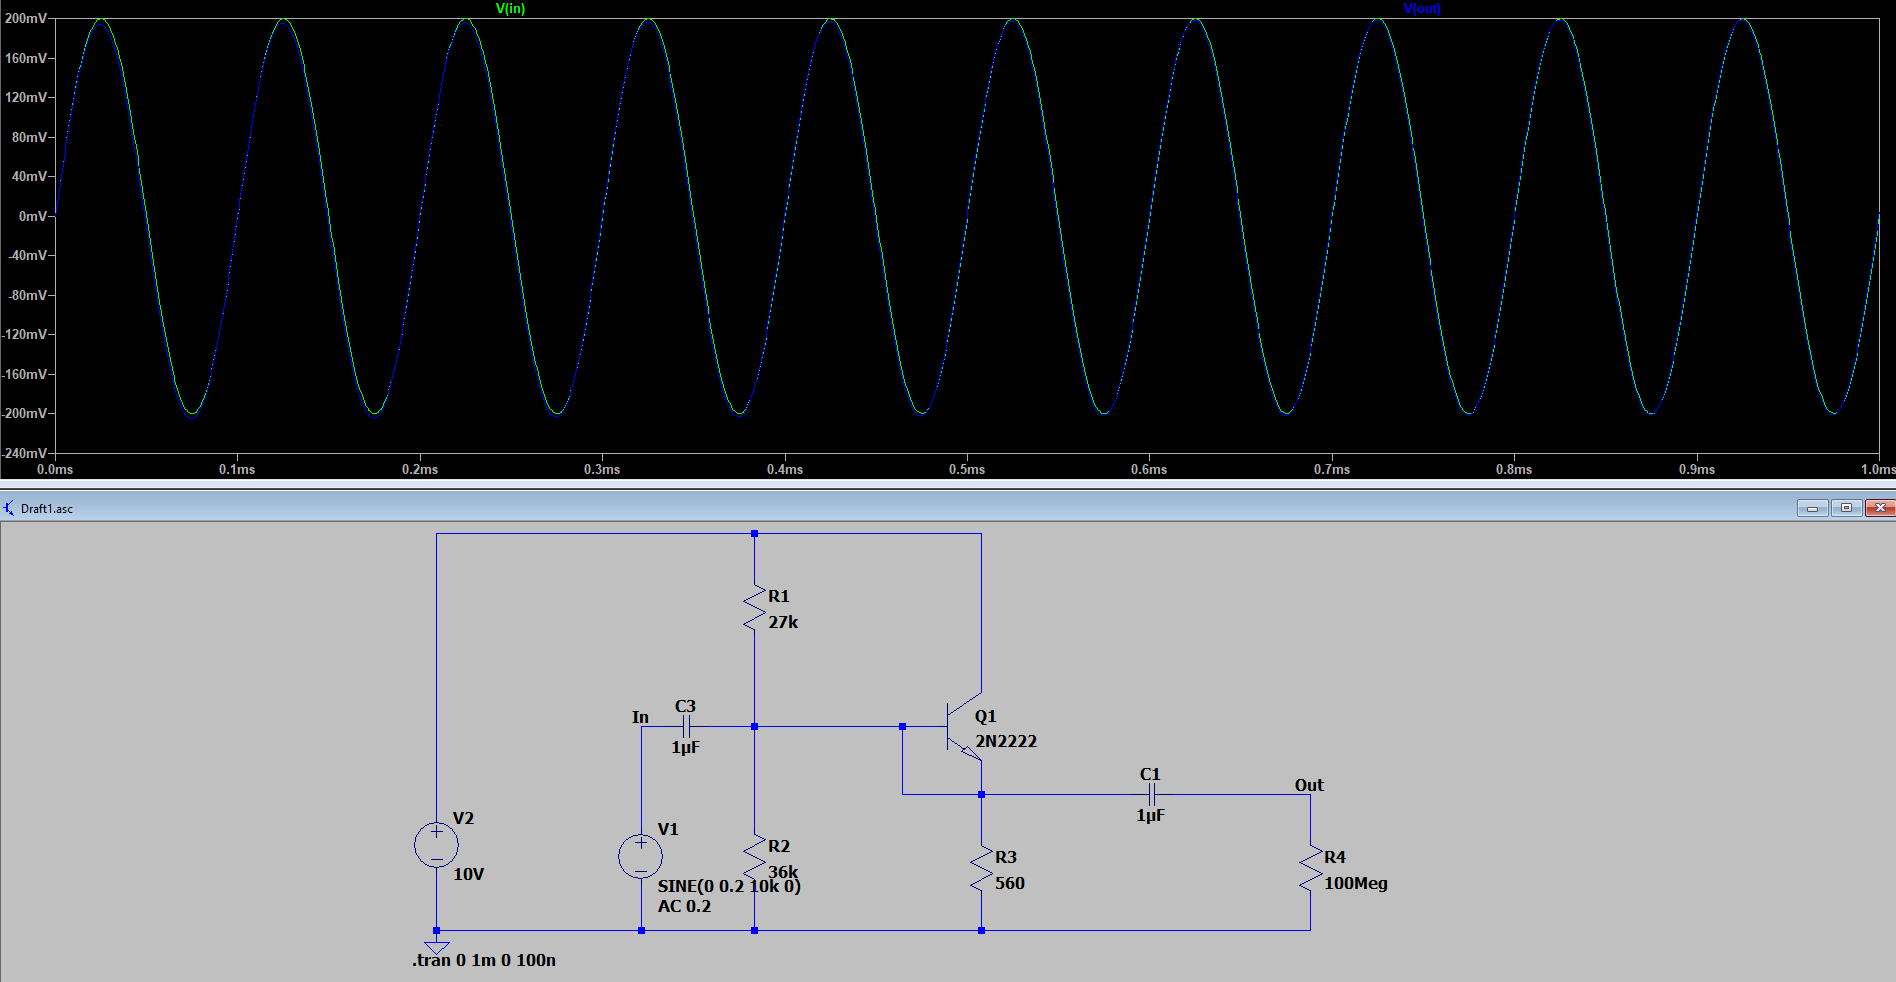
\includegraphics[width=\textwidth]{sim/ukol2/porucha4.png}
%   \caption{Simulace zkratu mezi bází a emitorem}
%   \label{fig:sch-sc-p5}
% \end{figure}

% \begin{figure}[H]
%   \centering
%   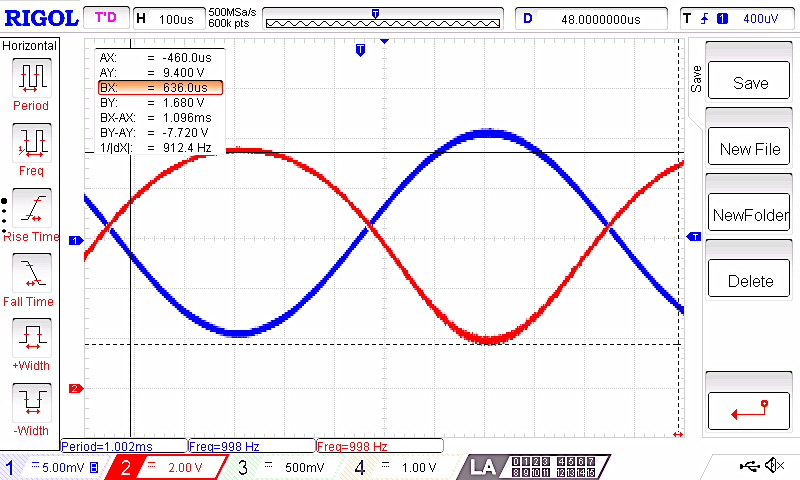
\includegraphics[width=0.95\textwidth]{mereni/NewFolder1/NewFile2.png}
%   \caption{Měření zkratu mezi bází a emitorem}
%   \label{fig:m-sch-sc-p5}
% \end{figure}

% % ---------------------------------------------------------------------------------

% \begin{figure}[H]
%   \centering
%   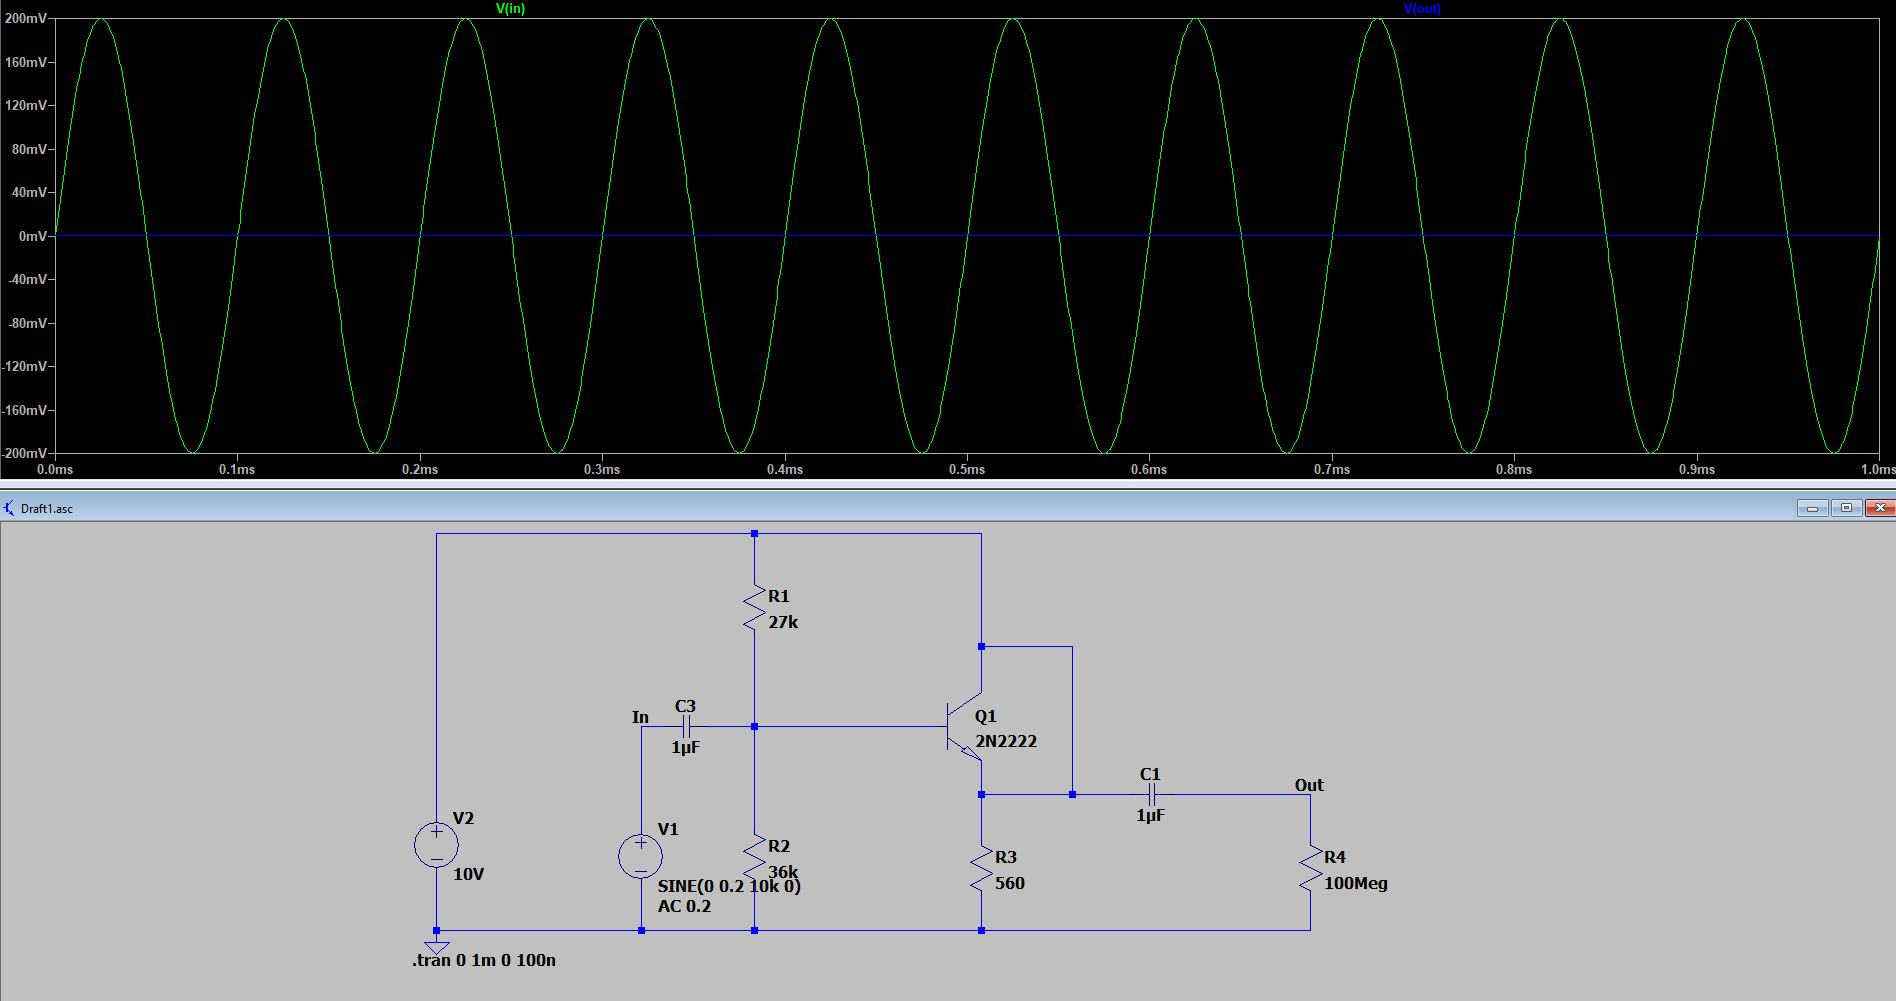
\includegraphics[width=\textwidth]{sim/ukol2/porucha5.png}
%   \caption{Simulace zkratu mezi kolektorem a emitorem}
%   \label{fig:sch-sc-p6}
% \end{figure}

% \begin{figure}[H]
%   \centering
%   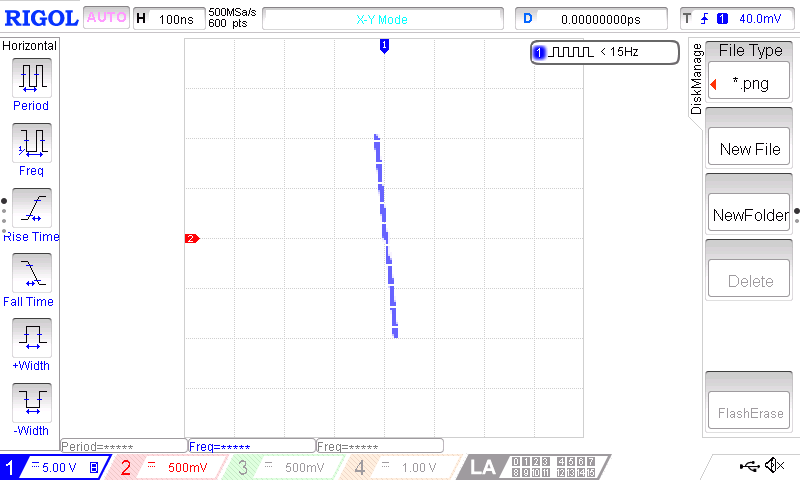
\includegraphics[width=0.95\textwidth]{mereni/NewFolder1/NewFile14.png}
%   \caption{Měření zkratu mezi kolektorem a emitorem}
%   \label{fig:m-sch-sc-p6}
% \end{figure}

% ---------------------------------------------------------------------------------



% \\ \\

% \subsection**{Měření kapacity \(C\)}
% Kapacitu kondenzátoru lze změřit pomocí měření průběhu jeho napětí při jeho vybíjení známým proudem.
% Pro jednoduchost tedy použijeme zdroj konstantního proudu o hodnotě \(I = 1\-[A]\) a následně na změřeném průběhu vybereme lineární část vybíjení (tedy tu kde se kondenzátor skutečně vybíjel požadovaným proudem).
% Kapacitu kondenzátoru můžeme následně určit jako:
% \\ \\
% \Large
% \(
%   C = \frac{t\cdot \Delta U}{I}
% \)
% \normalsize
% \\ \\

% \begin{figure}[H]
%   \begin{minipage}[t]{\textwidth}
%     \subsubsection*{Naše měření}
%     Pro všechny kondenzátory byl vybíjecí proud \(I = 1\-[A]\)
%     \begin{table}[H]
%       % \vspace{-75mm}
%       \centering
%       \begin{tabular}{|c|c|c||c|c|}
%         \hline
%                     &	\(\Delta U\-[V]\)  & \(t\-[s]\)   & \(C\-[F]\)  & katalogová hodnota \(C\)  \\ \hline
%           Maxwell   & 1.00               & 9.48         & 9.48        & \(8 \leq C \leq 10\)      \\ \hline
%           Eaton     & 1.00               & 8.36         & 8.36        & \(9 \leq C \leq 13\)      \\ \hline
%           Nichicon  & 1.00               & 8.4          & 8.4         & \(8 \leq C \leq 12\)      \\ \hline
%       \end{tabular}
%       \caption{\label{C} Změřené, vypočtené a výrobcem určené hodnoty k úkolu 2}
%     \end{table}
%     Příklad výpočtu:
%     \\ \\
%     \Large
%     \(
%       C = \frac{t\cdot \Delta U}{I} = \frac{9.48 \cdot 1}{1}\-[F]=9.48\-[\Omega]
%     \)
%     \normalsize
%     \\ \\
%     Z našeho měření kapacity plyne, že kapacita kondenzátorů je v toleranci určené výrobcem u kondenzátorů Maxwell a Nichicon, zatím co kondenzátor Eaton pravděpodobně vlivem stáří svojí kapacitu snížil pod úroveň výrobcem určeného intervalu.  
%   \end{minipage}
% \end{figure}

% \subsection**{Měření paralelního odporu \(R_P\)}
% Paralelní odpor způsobuje vybíjení kondenzátoru proudem \(I_L\).
% Hodnotu \(I_L\) můžeme určit z poklesu napětí na odporu, ze kterého není odebírán žádný proud za čas \(t\).
% \(I_L\) tak můžeme určit jako:
% \\ \\
% \Large
% \(
%   I_L = \frac{C\cdot \Delta U}{t}
% \)
% \normalsize
% \\ \\

% \begin{figure}[H]
%   \begin{minipage}[t]{\textwidth}
%     \subsubsection*{Naše měření}
%     Každý z kondenzátorů byl nabit na \(U_{AMP} = 2.2\-[V]\) a ponechán v nepřipojeném stavu po dobu 15 minut
%     \begin{table}[H]
%       % \vspace{-75mm}
%       \centering
%       \begin{tabular}{|c|c|c||c|c|}
%       \hline
%                   &	\(U\-[V]\) & \(I_L \-[mA]\) & katalogová hodnota \(I_L\-[mA]\)  \\ \hline
%         Maxwell   & 2.144      & 0.590          & 0.030                             \\ \hline
%         Eaton     & 2.067      & 1.235          & 0.023                             \\ \hline
%         Nichicon  & 2.072      & 1.195          & 5                                 \\ \hline
%       \end{tabular}
%       \caption{\label{U_AMP} Změřené, vypočtené a výrobcem určené hodnoty k úkolu 3}
%     \end{table}
%     Příklad výpočtu:
%     \\ \\
%     \Large
%     \(
%       I_L = \frac{C\cdot \Delta U}{t} = \frac{9.48\cdot 0.56}{15\cdot 60}\-[A]=0.0005899\-[A] = 0.5899\-[mA]
%     \)
%     \normalsize
%     \\ \\
%     Z našeho měření plyne, že jen kondenzátor Nichicon má hodnotu \(I_L\) v toleranci určené výrobcem zatím co u kondenzátorů Maxwell a Eaton jsme naměřili svodový proud řádově vyšší.
%     Vzhledem k velké odchylce od katalogové hodnoty je pravděpodobné, že došlo k chybě měření.  
%   \end{minipage}
% \end{figure}

% \subsection**{Závěr}

% \begin{figure}[H]
%   \begin{minipage}[t]{\textwidth}
%     \begin{table}[H]
%       \vspace{-10mm}
%       \centering
%       \begin{tabular}{|c|c|c|c|}
%         \hline
%                     & \(R_{ESR}\-[m\Omega]\) & \(C\-[F]\) & \(I_L \-[mA]\) \\ \hline
%           Maxwell   & 159.5                  & 9.48       & 0.590          \\ \hline
%           Eaton     & 156.9                  & 8.36       & 1.235          \\ \hline
%           Nichicon  & 162.2                  & 8.4        & 1.195          \\ \hline
%       \end{tabular}
%       \caption{\label{Vysledky} Výsledky měření}
%     \end{table}
%     \vspace{-10mm}
%   \end{minipage}
% \end{figure}

% \subsection**{Měření \(R_{ESR}\)}
% Naše měření bylo buď zatíženo podstatnou chybou metody nebo je skutečný odpor kondenzátorů \(R_{ESR}\) velmi výrazně nad limity stanovenými výrobcem. 
% \subsection**{Měření kapacity \(C\)}
% Z našeho měření kapacity plyne, že kapacita kondenzátorů je v toleranci určené výrobcem u kondenzátorů Maxwell a Nichicon, zatím co kondenzátor Eaton pravděpodobně vlivem stáří svojí kapacitu snížil pod úroveň výrobcem určeného intervalu.
% \subsection**{Měření paralelního odporu \(R_P\)}
% Z našeho měření plyne že jen kondenzátor Nichicon má hodnotu \(I_L\) v toleranci určené výrobcem zatím co u kondenzátorů Maxwell a Eaton jsme naměřili svodový proud řádově vyšší.
% Vzhledem k velké odchylce od katalogové hodnoty je pravděpodobné, že došlo k chybě měření.

\end{document}